
%% bare_conf.tex
%% V1.4b
%% 2015/08/26
%% by Michael Shell
%% See:
%% http://www.michaelshell.org/
%% for current contact information.
%%
%% This is a skeleton file demonstrating the use of IEEEtran.cls
%% (requires IEEEtran.cls version 1.8b or later) with an IEEE
%% conference paper.
%%
%% Support sites:
%% http://www.michaelshell.org/tex/ieeetran/
%% http://www.ctan.org/pkg/ieeetran
%% and
%% http://www.ieee.org/

%%*************************************************************************
%% Legal Notice:
%% This code is offered as-is without any warranty either expressed or
%% implied; without even the implied warranty of MERCHANTABILITY or
%% FITNESS FOR A PARTICULAR PURPOSE! 
%% User assumes all risk.
%% In no event shall the IEEE or any contributor to this code be liable for
%% any damages or losses, including, but not limited to, incidental,
%% consequential, or any other damages, resulting from the use or misuse
%% of any information contained here.
%%
%% All comments are the opinions of their respective authors and are not
%% necessarily endorsed by the IEEE.
%%
%% This work is distributed under the LaTeX Project Public License (LPPL)
%% ( http://www.latex-project.org/ ) version 1.3, and may be freely used,
%% distributed and modified. A copy of the LPPL, version 1.3, is included
%% in the base LaTeX documentation of all distributions of LaTeX released
%% 2003/12/01 or later.
%% Retain all contribution notices and credits.
%% ** Modified files should be clearly indicated as such, including  **
%% ** renaming them and changing author support contact information. **
%%*************************************************************************


% *** Authors should verify (and, if needed, correct) their LaTeX system  ***
% *** with the testflow diagnostic prior to trusting their LaTeX platform ***
% *** with production work. The IEEE's font choices and paper sizes can   ***
% *** trigger bugs that do not appear when using other class files.       ***                          ***
% The testflow support page is at:
% http://www.michaelshell.org/tex/testflow/



\documentclass[journal,final,twocolumn]{IEEEtran}
\usepackage{mathrsfs}
\usepackage{amsmath}
\usepackage{amsthm}
\usepackage{amssymb}
\usepackage{cite}
\usepackage{amsfonts}
\usepackage{graphicx}
\usepackage{subfigure}
\usepackage{bm}
\usepackage{diagbox} 
\usepackage{enumerate}
\usepackage{indentfirst}
\usepackage[colorlinks ,linkcolor=blue]{hyperref}
\newtheorem{remark}{Remark}
\newtheorem{theorem}{Theorem}
\newtheorem{definition}{Definition} 
\newtheorem{assumption}{Assumption}
\newtheorem{algorithm}{Algorithm}

\allowdisplaybreaks 
% *** CITATION PACKAGES ***
%
%\usepackage{cite}
% cite.sty was written by Donald Arseneau
% V1.6 and later of IEEEtran pre-defines the format of the cite.sty package
% \cite{} output to follow that of the IEEE. Loading the cite package will
% result in citation numbers being automatically sorted and properly
% "compressed/ranged". e.g., [1], [9], [2], [7], [5], [6] without using
% cite.sty will become [1], [2], [5]--[7], [9] using cite.sty. cite.sty's
% \cite will automatically add leading space, if needed. Use cite.sty's
% noadjust option (cite.sty V3.8 and later) if you want to turn this off
% such as if a citation ever needs to be enclosed in parenthesis.
% cite.sty is already installed on most LaTeX systems. Be sure and use
% version 5.0 (2009-03-20) and later if using hyperref.sty.
% The latest version can be obtained at:
% http://www.ctan.org/pkg/cite
% The documentation is contained in the cite.sty file itself.






% *** GRAPHICS RELATED PACKAGES ***
%
\ifCLASSINFOpdf
  % \usepackage[pdftex]{graphicx}
  % declare the path(s) where your graphic files are
  % \graphicspath{{../pdf/}{../jpeg/}}
  % and their extensions so you won't have to specify these with
  % every instance of \includegraphics
  % \DeclareGraphicsExtensions{.pdf,.jpeg,.png}
\else
  % or other class option (dvipsone, dvipdf, if not using dvips). graphicx
  % will default to the driver specified in the system graphics.cfg if no
  % driver is specified.
  % \usepackage[dvips]{graphicx}
  % declare the path(s) where your graphic files are
  % \graphicspath{{../eps/}}
  % and their extensions so you won't have to specify these with
  % every instance of \includegraphics
  % \DeclareGraphicsExtensions{.eps}
\fi
% graphicx was written by David Carlisle and Sebastian Rahtz. It is
% required if you want graphics, photos, etc. graphicx.sty is already
% installed on most LaTeX systems. The latest version and documentation
% can be obtained at: 
% http://www.ctan.org/pkg/graphicx
% Another good source of documentation is "Using Imported Graphics in
% LaTeX2e" by Keith Reckdahl which can be found at:
% http://www.ctan.org/pkg/epslatex
%
% latex, and pdflatex in dvi mode, support graphics in encapsulated
% postscript (.eps) format. pdflatex in pdf mode supports graphics
% in .pdf, .jpeg, .png and .mps (metapost) formats. Users should ensure
% that all non-photo figures use a vector format (.eps, .pdf, .mps) and
% not a bitmapped formats (.jpeg, .png). The IEEE frowns on bitmapped formats
% which can result in "jaggedy"/blurry rendering of lines and letters as
% well as large increases in file sizes.
%
% You can find documentation about the pdfTeX application at:
% http://www.tug.org/applications/pdftex





% *** MATH PACKAGES ***
%
%\usepackage{amsmath}
% A popular package from the American Mathematical Society that provides
% many useful and powerful commands for dealing with mathematics.
%
% Note that the amsmath package sets \interdisplaylinepenalty to 10000
% thus preventing page breaks  from occurring within multiline equations. Use:
%\interdisplaylinepenalty=2500
% after loading amsmath to restore such page breaks  as IEEEtran.cls normally
% does. amsmath.sty is already installed on most LaTeX systems. The latest
% version and documentation can be obtained at:
% http://www.ctan.org/pkg/amsmath





% *** SPECIALIZED LIST PACKAGES ***
%
%\usepackage{algorithmic}
% algorithmic.sty was written by Peter Williams and Rogerio Brito.
% This package provides an algorithmic environment fo describing algorithms.
% You can use the algorithmic environment in-text or within a figure
% environment to provide for a floating algorithm. Do NOT use the algorithm
% floating environment provided by algorithm.sty (by the same authors) or
% algorithm2e.sty (by Christophe Fiorio) as the IEEE does not use dedicated
% algorithm float types and packages that provide these will not provide
% correct IEEE style captions. The latest version and documentation of
% algorithmic.sty can be obtained at:
% http://www.ctan.org/pkg/algorithms
% Also of interest may be the (relatively newer and more customizable)
% algorithmicx.sty package by Szasz Janos:
% http://www.ctan.org/pkg/algorithmicx




% *** ALIGNMENT PACKAGES ***
%
%\usepackage{array}
% Frank Mittelbach's and David Carlisle's array.sty patches and improves
% the standard LaTeX2e array and tabular environments to provide better
% appearance and additional user controls. As the default LaTeX2e table
% generation code is lacking to the point of almost being broken with
% respect to the quality of the end results, all users are strongly
% advised to use an enhanced (at the very least that provided by array.sty)
% set of table tools. array.sty is already installed on most systems. The
% latest version and documentation can be obtained at:
% http://www.ctan.org/pkg/array


% IEEEtran contains the IEEEeqnarray family of commands that can be used to
% generate multiline equations as well as matrices, tables, etc., of high
% quality.




% *** SUBFIGURE PACKAGES ***
%\ifCLASSOPTIONcompsoc
%  \usepackage[caption=false,font=normalsize,labelfont=sf,textfont=sf]{subfig}
%\else
%  \usepackage[caption=false,font=footnotesize]{subfig}
%\fi
% subfig.sty, written by Steven Douglas Cochran, is the modern replacement
% for subfigure.sty, the latter of which is no longer maintained and is
% incompatible with some LaTeX packages including fixltx2e. However,
% subfig.sty requires and automatically loads Axel Sommerfeldt's caption.sty
% which will override IEEEtran.cls' handling of captions and this will result
% in non-IEEE style figure/table captions. To prevent this problem, be sure
% and invoke subfig.sty's "caption=false" package option (available since
% subfig.sty version 1.3, 2005/06/28) as this is will preserve IEEEtran.cls
% handling of captions.
% Note that the Computer Society format requires a larger sans serif font
% than the serif footnote size font used in traditional IEEE formatting
% and thus the need to invoke different subfig.sty package options depending
% on whether compsoc mode has been enabled.
%
% The latest version and documentation of subfig.sty can be obtained at:
% http://www.ctan.org/pkg/subfig




% *** FLOAT PACKAGES ***
%
%\usepackage{fixltx2e}
% fixltx2e, the successor to the earlier fix2col.sty, was written by
% Frank Mittelbach and David Carlisle. This package corrects a few problems
% in the LaTeX2e kernel, the most notable of which is that in current
% LaTeX2e releases, the ordering of single and double column floats is not
% guaranteed to be preserved. Thus, an unpatched LaTeX2e can allow a
% single column figure to be placed prior to an earlier double column
% figure.
% Be aware that LaTeX2e kernels dated 2015 and later have fixltx2e.sty's
% corrections already built into the system in which case a warning will
% be issued if an attempt is made to load fixltx2e.sty as it is no longer
% needed.
% The latest version and documentation can be found at:
% http://www.ctan.org/pkg/fixltx2e


%\usepackage{stfloats}
% stfloats.sty was written by Sigitas Tolusis. This package gives LaTeX2e
% the ability to do double column floats at the bottom of the page as well
% as the top. (e.g., "\begin{figure*}[!b]" is not normally possible in
% LaTeX2e). It also provides a command:
%\fnbelowfloat
% to enable the placement of footnotes below bottom floats (the standard
% LaTeX2e kernel puts them above bottom floats). This is an invasive package
% which rewrites many portions of the LaTeX2e float routines. It may not work
% with other packages that modify the LaTeX2e float routines. The latest
% version and documentation can be obtained at:
% http://www.ctan.org/pkg/stfloats
% Do not use the stfloats baselinefloat ability as the IEEE does not allow
% \baselineskip to stretch. Authors submitting work to the IEEE should note
% that the IEEE rarely uses double column equations and that authors should try
% to avoid such use. Do not be tempted to use the cuted.sty or midfloat.sty
% packages (also by Sigitas Tolusis) as the IEEE does not format its papers in
% such ways.
% Do not attempt to use stfloats with fixltx2e as they are incompatible.
% Instead, use Morten Hogholm'a dblfloatfix which combines the features
% of both fixltx2e and stfloats:
%
% \usepackage{dblfloatfix}
% The latest version can be found at:
% http://www.ctan.org/pkg/dblfloatfix




% *** PDF, URL AND HYPERLINK PACKAGES ***
%
%\usepackage{url}
% url.sty was written by Donald Arseneau. It provides better support for
% handling and breaking URLs. url.sty is already installed on most LaTeX
% systems. The latest version and documentation can be obtained at:
% http://www.ctan.org/pkg/url
% Basically, \url{my_url_here}.




% *** Do not adjust lengths that control margins, column widths, etc. ***
% *** Do not use packages that alter fonts (such as pslatex).         ***
% There should be no need to do such things with IEEEtran.cls V1.6 and later.
% (Unless specifically asked to do so by the journal or conference you plan
% to submit to, of course. )


% correct bad hyphenation here
\hyphenation{op-tical net-works  semi-conduc-tor}


\begin{document}
%
% paper title
% Titles are generally capitalized except for words such as a, an, and, as,
% at, but, by, for, in, nor, of, on, or, the, to and up, which are usually
% not capitalized unless they are the first or last word of the title.
% Linebreaks  \\ can be used within to get better formatting as desired.
% Do not put math or special symbols in the title.
\title{Asynchronous Sliding Mode Control of Two-Dimensional Markov Jump Systems}


% author names and affiliations
% use a multiple column layout for up to three different
% affiliations
%\author{\IEEEauthorblockN{Michael Shell}
%\IEEEauthorblockA{School of Electrical and\\Computer Engineering\\
%Georgia Institute of Technology\\
%Atlanta, Georgia 30332--0250\\
%Email: http://www.michaelshell.org/contact.html}
%\and
%\IEEEauthorblockN{Homer Simpson}
%\IEEEauthorblockA{Twentieth Century Fox\\
%Springfield, USA\\
%Email: homer@thesimpsons.com}
%\and
%\IEEEauthorblockN{James Kirk\\ and Montgomery Scott}
%\IEEEauthorblockA{Starfleet Academy\\===
%San Francisco, California 96678--2391\\
%Telephone: (800) 555--1212\\
%Fax: (888) 555--1212}}

% conference papers do not typically use \thanks  and this command
% is locked out in conference mode. If really needed, such as for
% the acknowledgment of grants, issue a \IEEEoverridecommandlockouts
% after \documentclass

% for over three affiliations, or if they all won't fit within the width
% of the page, use this alternative format:
% 
%\author{\IEEEauthorblockN{Michael Shell\IEEEauthorrefmark{1},
%Homer Simpson\IEEEauthorrefmark{2},
%James Kirk\IEEEauthorrefmark{3}, 
%Montgomery Scott\IEEEauthorrefmark{3} and
%Eldon Tyrell\IEEEauthorrefmark{4}}
%\IEEEauthorblockA{\IEEEauthorrefmark{1}School of Electrical and Computer Engineering\\
%Georgia Institute of Technology,
%Atlanta, Georgia 30332--0250\\ Email: see http://www.michaelshell.org/contact.html}
%\IEEEauthorblockA{\IEEEauthorrefmark{2}Twentieth Century Fox, Springfield, USA\\
%Email: homer@thesimpsons.com}
%\IEEEauthorblockA{\IEEEauthorrefmark{3}Starfleet Academy, San Francisco, California 96678-2391\\
%Telephone: (800) 555--1212, Fax: (888) 555--1212}
%\IEEEauthorblockA{\IEEEauthorrefmark{4}Tyrell Inc., 123 Replicant Street, Los Angeles, California 90210--4321}}

%\author{\IEEEauthorblockN{Yue-Yue Tao, Zheng-Guang Wu, and Peng Shi }}

\author{Yue-Yue Tao, Zheng-Guang Wu, and Peng Shi
%	\thanks{ This work was supported by the Fundamental Research Funds for the Central Universities (Grant no. 2018FZA5009), the National Science Foundation (Grant no. ECCS-1611423) and the China Scholarship Council (Grant no. 201706320267). Corresponding author:~Wei~Ren.}
	\thanks{Y. Tao and Z.-G. Wu are with the National Laboratory of Industrial Control Technology, Institute of Cyber-Systems and Control, Zhejiang University, Hangzhou Zhejiang, 310027, PR China (e-mail: taoyueyue54@zju.edu.cn; nashwzhg@zju.edu.cn).}
	\thanks{P. Shi is with the School of Electrical and Electronic Engineering, University of Adelaide, Adelaide, SA 5005, Australia (e-mail: peng.shi@adelaide.edu.au). }  
}

% use for special paper notices
%\IEEEspecialpapernotice{(Invited Paper)}
\markboth{IEEE}%
{Shell \MakeLowercase{\textit{et al.}}: Bare Demo of IEEEtran.cls for Journals}

% make the title area
\maketitle



% As a general rule, do not put math, special symbols or citations
% in the abstract
\begin{abstract}
	In this paper, asynchronous sliding mode control (SMC) is investigated for two-dimensional (2D) discrete-time Markov jump systems. As the system modes are not always accessible to the controller, the hidden Markov model is employed to describe the asynchronization between the system models and controller. A new 2D sliding surface is constructed and the corresponding asynchronous SMC is designed under the framework of hidden Markov model. By Lyapunov function and linear matrix inequality (LMI) approaches, sufficient conditions are presented to guarantee the underlying 2D system is asymptotically mean square stable (AMSS) with an $H_\infty$ disturbance attenuation performance. Then, an algorithm is provided to derive the asynchronous 2D-SMC law. Finally, an example is given to verify the validity and effectiveness of the new SMC law design algorithm.
\end{abstract}

% no keywords

\begin{IEEEkeywords}
	Markov jump systems, 2D systems, sliding mode control, hidden Markov model
\end{IEEEkeywords}



% For peer review papers, you can put extra information on the cover
% page as needed:
% \ifCLASSOPTIONpeerreview
% \begin{center} \bfseries EDICS Category: 3-BBND \end{center}
% \fi
%
% For peerreview papers, this IEEEtran command inserts a page break and
% creates the second title. It will be ignored for other modes.
\IEEEpeerreviewmaketitle
  
   

\section{Introduction}
	Markov jump systems (MJSs), a special class of stochastic switching systems, have received considerable attentions for its powerful ability in modeling systems with sudden changes in parameters or system structures, for instance,  environmental disturbances, actuator failures, and interconnection variations in subsystems, etc. Over the past decades, a large number of results on system stability analysis and  design of controllers/filters have been reported in \cite{costa2006discrete, wu2014asynchronous, zhang2008analysis, shi2006designing, zhang2009stability}.
	
	However, the aforementioned works  are generally based on the implicit assumption that the information of system modes are always  fully available for the controller/filter, so that the controller/filter modes can run synchronously with system modes. Unfortunately, in practical applications, it is rather difficult to satisfy this ideal assumption because of some unexpected factors, such as, time delays, data dropouts and quantization in networked control systems. To overcome the strict limitation, two research approaches were proposed, namely, mode-independent and asynchronous methods. In mode-independent methods, see \cite{todorov2016new,wu2005mode,dolgov2017static}, the controller/filter modes are independent of system modes, which means the information of system modes is not fully utilized and may result in some conservativeness. In \cite{wu2016passivity}, Wu proposed the hidden Markov model, a united asynchronous framework that covers synchronous and mode-independent cases. A similar description of this model can also be found in earlier works \cite{costa2006discrete} and \cite{do2014detector}. The hidden Markov model supposes that the controller/filter modes can be detected via a hidden Markov chain, such that controllers/filters can utilize more information of the origin system modes.  Base on this model, many problems of asynchronous control/filtering for MJSs have been studied in recent years \cite{de2017h,todorov2018detector,rodrigues2018detector}. 
	
	
	Moreover, SMC, an effective control technique for its strong robustness against parameter variations,  exogenous disturbances and model uncertainties, has been successfully applied to a large variety of practical systems \cite{utkin2009sliding,yang1999sliding,shima2006sliding}.  The prime idea of SMC is to design a discontinuous control law to drive the system state trajectories toward a predefined sliding surface and stay within a neighbourhood of the  sliding surface after reaching it \cite{edwards1998sliding}. In the last few decades, the SMC design problems have been extensively studied, and a large number of  research results for MJSs have been published \cite{li2015state,wu2010state,wang2017smc}. Recently, some researchers have investigated the asynchronous SMC design methods for one-dimensional (1D) MJSs based on hidden Markov model \cite{song2018asynchronous,li2017passivity,qi2018observer}. 
	
	
	On the other hand, 2D systems, a special class of multi-dimensional systems  dating back to 1970s,  have been used to represent a large variety of practical applications, such as digital image processing, partial differential equations modeling and signal filtering \cite{roesser1975discrete,marszalek1984two,rogers2015multidimensional}, etc. Different from 1D systems, the prime feature of  2D systems lie in the system information propagates along two different directions and the information in each direction will have effects on the other, which brings much complexity and difficulty in system analysis and synthesis. To describe the special properties of 2D systems, several  mathematical models presented in state-space framework have been proposed, for example Roesser model \cite{roesser1975discrete} and Fornasini-Marchesini model \cite{fornasini1978doubly}. In Roesser model, the system state is composed of two independent states, horizontal state and vertical state, which are denoted by  sub-vectors, the next horizontal state and vertical state in different directions can be deduced from current state, respectively. Unlike the Roesser model, the system state in Fornasini-Marchesini model is represented by a vector which is a function with two independent variables, and the current system state is derived from the  last two adjacent states in different directions. In most circumstances, Roesser model can be regarded as particular case of Fornasini-Marchesini model, but is much simpler and more intelligible than the latter. Based on 2D bounded real lemma, the $H_{\infty}$ control theory for 2D systems was established by Du and Xie in \cite{du2001h} and \cite{du2002hinfinity}. This result was extended to control and filtering problems for 2D systems with time-varying delays \cite{trinh2016stability},  multiplicative noise \cite{ahn2016stochastic} and uncertainty parameters \cite{chesi2016robust}. 
	Anh has studied  the dissipative control and filtering problems for 2D systems in \cite{ahn2015two}  by utilizing linear matrix inequalities technique.
	A large number of preliminary results on SMC of discrete-time 2D systems have been established \cite{liu2005adaptive,wu2008sliding,yang2019two}.
	In recent years, 2D systems with Markov jump parameters have attracted more interests of researchers. For example,  the $H_{\infty}$ control, $H_{\infty}$ filtering, $H_{\infty}$ mode reduction and fault detection problems for 2D-MJSs have been investigated in \cite{gao2004stabilization,wu2018hcontrol2d,wu2008hfiltering2d,wu2006modelreduction,shen2019dissipativity}, respectively. However, we have to notice that, the issue of SMC  for 2D-MJSs has not been studied yet, which motivates us for current work.
	 
	Based on the aforementioned considerations, we will investigate the problem of asynchronous SMC for 2D-MJSs in this paper. 
	The primary contributions of this paper are shown as following aspects:
	\begin{enumerate}
		\item Based on the structural properties of 2D systems, a novel 2D sliding surface is constructed, and the corresponding asynchronous 2D-SMC law is designed under the framework of hidden Markov model, which means it is more practical and flexible than the synchronous or mode-independent ones.
		\item  A sufficient condition that can guarantee the concerned 2D system is AMSS with an  $H_{\infty}$ disturbance attenuation performance is established. Moreover, this condition can simultaneously ensure the reachability of the sliding mode dynamics. Finally, the  design procedures of SMC law are summarized into an algorithm. 
		\item Though asynchronous SMC schemes for 1D-MJSs have been extensively studied in previous works, such as \cite{song2018asynchronous,li2017passivity,qi2018observer} etc. However, the results of those works can't directly applied to 2D-MJSs for its complex structural properties. It is the first time that the asynchronous SMC is investigated for 2D-MJSs, which shows the feasibility and effectiveness of SMC for 2D-MJSs.   
	\end{enumerate}

\section{Preliminaries} \label{priliminaries}
	Considering the following discrete-time 2D-MJS in Roesser model:
	\begin{equation} \label{system-equation}
	\left\{
		\begin{array}{lr}
			\begin{split}
				\emph{\textbf{x(i, j)}} &= A_{r(i,j)}x(i,j)+E_{r(i,j)}w(i,j)\\
										&+B_{r(i,j)}[(u(i,j)+f(x(i,j),r(i,j))]
			\end{split}\\
			\begin{split}
				y(i,j) = C_{r(i,j)}x(i,j)+D_{r(i,j)}w(i,j)
			\end{split}
		\end{array}
	\right.
	\end{equation}
	where
	\begin{equation*}
		\emph{\textbf{x(i, j)}} = \begin{bmatrix}
			x^{h}(i+1,j)\\
			x^{v}(i,j+1)
		\end{bmatrix}, \ 
		x(i, j) = \begin{bmatrix}
		x^{h}(i,j)\\
		x^{v}(i,j)
		\end{bmatrix}          
	\end{equation*}
	$x^{h}(i,j)\in \mathbb{R}^{n_h}$ and $x^{v}(i,j)\in \mathbb{R}^{n_v}$ represent horizontal and vertical sub-states respectively, $u(i,j) \in \mathbb{R}^{n_u}$ and $y(i,j) \in \mathbb{R}^{n_y}$ represent the control input and controlled output respectively, and $w(i,j) \in \mathbb{R}^{n_w}$ represents the exogenous disturbance which belongs to $\ell_{2}\{[0,\infty),[0,\infty)\}$. $A_{r(i,j)}$, $B_{r(i,j)}$, $C_{r(i,j)}$, $D_{r(i,j)}$ and $E_{r(i,j)}$ represent the time-varying system matrices, all of which are real known with appropriate dimensions. Besides, we assume that the matrix $B_{r(i,j)}$ is full column rank for each $r(i,j)\in\mathcal{N}_{1}$, that is, rank($B_{r(i,j)}$)$=n_u$. The nonlinear function $f(x(i,j),r(i,j))$ satisfies the following property:
	\begin{equation}\label{nonlinear-func}
		\|f(x(i,j),r(i,j)\| \leq \delta_{r(i,j)}\|x(i,j)\|
	\end{equation}
	where $\delta_{r(i,j)}$ is a known scalar, $\|\cdot\|$ denotes the Euclidean norm of a vector. The parameter $r(i,j)$ takes values in a finite set $\mathcal{N}_{1}=\{1,2...,N_{1} \}$ with transition probability matrix $\varLambda = [\lambda_{kp}]$, and the related transition probability in both directions satisfies (see \cite{wu2018hcontrol2d,wu2008hfiltering2d})
%	\begin{equation}\label{tps_system}
%	\begin{split}
%	&\Pr\{r(i+1,j)=p|r(i,j)=k\}\\
%	=&\Pr\{r(i,j+1)=p|r(i,j)=k\}=\lambda_{kp},\  \forall k,p \in \mathcal{N}_{1}
%	\end{split}
%	\end{equation}
	\begin{equation}\label{tps_system}
	\lambda_{kp}=
	\begin{cases}
	\Pr\{r(i+1,j)=p|r(i,j)=k\},\\
	\Pr\{r(i,j+1)=p|r(i,j)=k\}, 
	\end{cases} \forall k,p \in \mathcal{N}_{1}
	\end{equation}
	where $\lambda_{kp}\in[0,1]$, for all $k, p\in\mathcal{N}_{1}$, and $\sum_{p=1}^{N_1}\lambda_{kp}=1$ for every mode $k$.
%	\begin{remark}
%		We should notice that condition \eqref{tps_system}  contains a implicit assumption, that is, mode transition probability from (i,j)  to (i+1,j) and (i,j+1) are equal. 
%	\end{remark}
	We define the boundary condition ($X_{0},\varGamma_{0}$) of the 2D-MJS \eqref{system-equation}, as follows:
	\begin{equation} \label{boundary-condition}
	\left\{
		\begin{array}{lr}
			\begin{split}
				X_{0} &= \{x^{h}(0,j),x^{v}(i,0)|\ i,j = 0,1,2...\}\\
				\varGamma_{0} &= \{r(0,j), r(i,0)|\ i,j = 0,1,2... \}
			\end{split}
		\end{array}
	\right.
	\end{equation}
	And the corresponding zero boundary condition is assumed as $x^{h}(0,j) =0, x^{v}(i,0)=0$, for every nonnegative integer $i,j$. Besides, the following assumption is imposed on $X_{0}$:
	
	\begin{assumption}\label{boundary-assumptin}
	 	The boundary condition $X_{0}$ satisfies:
	 	\begin{equation}
	 		\lim\limits_{Z\to\infty}\mathbb{E}\Big\{\sum_{z=0}^{Z}(\|x^{h}(0,z)\|^{2}+ \|x^{v}(z,0)\|^{2})\Big\} < \infty
	 	\end{equation}
	 	Here $\mathbb{E}\{\cdot\}$ represents the mathematical expectation.
	\end{assumption}
	
	In practical applications, the complete information of $r(i,j)$ can not always be available to the controller. Hence, in this paper, the hidden Markov model $(r(i,j),\sigma(i,j),\varLambda,\varPsi)$ as in \cite{wu2016passivity} is introduced to characterize the asynchronous phenomenon between the controller and the original system. The parameter $\sigma(i,j)$, refers to controller mode, takes values in another finite set $\mathcal{N}_{2} = \{1,2...N_{2}\}$, and satisfies the conditional probability matrix $\varPsi=[\mu_{k\tau} ]$ with conditional mode transition probabilities
	\begin{equation}
		\Pr\{\sigma(i,j)=\tau|r(i,j)=k\}=\mu_{k\tau } %\forall  k\in\mathcal{N}_{1}, \tau\in\mathcal{N}_{2}
	\end{equation}
	where $\mu_{k\tau }\in[0,1]$ for all $k\in\mathcal{N}_{1}, \tau\in\mathcal{N}_{2}$, and $\sum_{\tau =1}^{N_{2}}\mu_{k\tau } = 1$ for any mode $k$.
	
	\begin{remark}
		Two strict assumptions are required to guarantee the controller modes run synchronously with original system modes all the time. First, all system modes should be detected accurately by the controller in time. Second, the controller should switch to the corresponding mode in time. However, the first assumption might be impaired by  failures or delays of communication devices, and the second assumption might be impaired by failures or low efficiency of mode switching devices. In other words, the synchronous controller has high requirements on the reliability and efficiency of the physical equipment, which are rather difficult to be guaranteed.  Therefore, the mismatched modes between controller and system are more practical in real applications. The hidden Markov model can flexibly handle the mismatched modes between controller and system through statistical methods, which will reduce requirements for physical devices. 
	\end{remark}

 
\begin{remark}
	The hidden Markov model is a united framework that covers synchronous, asynchronous and mode-independent cases.  In this model, system modes are governed by the Markov chain $\{r(i,j), i,j=1,2\ \dots\}$, and controller modes are derived by the conditional mode transition probability $u_{k\tau}$. That is, the conditional probability matrix $\varPsi$ establishes a connection between the modes of controller and original system. Which case the controller belongs to depends on the conditional probability matrix $\varPsi$.  The controller becomes a synchronous one when $\varPsi$ is a unit matrix, or becomes a mode-independent one when $\mathcal{N}_{2}=\{1\}$. Thus, the established results  can be readily extended to synchronous or mode-independent  cases  by adjusting the conditional probability matrix $\varPsi$.
\end{remark}
	
	In the following, the definitions of  AMSS and $H_{\infty}$ disturbance attenuation performance for 2D systems will be given in Definition \ref{mean-square-stable} and Definition \ref{H_infty-performance}, respectively.
	
	\begin{definition}\label{mean-square-stable}
	For $w(i,j)\equiv0$, the 2D-MJS \eqref{system-equation} under Assumption \ref{boundary-assumptin} is said to be AMSS,  if the following formulation holds:
	\begin{equation}\label{AMSS}
			\lim\limits_{i+j\to\infty}\mathbb{E}\{\|x(i,j)\|^{2}\} = 0
	\end{equation}
	for any boundary condition $X_{0}$.
	\end{definition}

%	\begin{definition}\label{mean-square-stable}
%	If for $w(i,j)\equiv0$, boundary condition $(X_{0},\varGamma_{0})$, the following formulation holds:
%	\begin{equation}
%	\lim\limits_{i+j\to\infty}\mathbb{E}\{\|x(i,j)\|^{2}\} = 0
%	\end{equation}
%	then the 2D Markov jump system \eqref{system-equation} is said to be asymptotically mean square stable.
%	\end{definition}

	\begin{definition}\label{H_infty-performance}
		Given a scalar $\gamma>0$,  the 2D-MJS \eqref{system-equation} under zero boundary condition with $w(i,j)\in \ell_{2}\{[0,\infty),[0,\infty)\}$ is said to be AMSS with an $H_{\infty}$ disturbance attenuation performance $\gamma$. if \eqref{AMSS} and following formulation hold:
		\begin{equation} \label{invDef2}
			\sum_{i=0}^{\infty}\sum_{j=0}^{\infty}\mathbb\{\|y(i,j)\|^{2}\} <  \gamma^{2} \sum_{i=0}^{\infty}\sum_{j=0}^{\infty}\mathbb\{\|w(i,j)\|^{2}\}.
		\end{equation}
	\end{definition}
	
	Now, we will make some notational simplification for convenience. The parameter $r(i,j)$ will be represented by $k$, and $\sigma(i,j)$ will be represented by $\tau$. 
	
	 The objective of this work is to design an asynchronous  2D-SMC law, such that the 2D-MJS \eqref{system-equation} is AMSS with an $H_{\infty}$ disturbance attenuation performance $\gamma$. 

\section{Main Result}
In this section, we first construct a novel 2D sliding surface based on the properties of 2D systems, and design an  corresponding  asynchronous 2D-SMC law under hidden Markov model.  Then, we will analyze the asymptotic mean square stability for the concerned 2D-MJS and the reachability of the sliding mode dynamics.

\subsection{ Sliding Surface and Asynchronous SMC Law Design} \label{sliding-surface}
	In this work, we construct a novel 2D sliding surface as follows: 
	\begin{equation}\label{siding-surface-equation}	
		s(i,j) = \begin{bmatrix}
					s^{h}(i,j)\\
					s^{v}(i,j)
					\end{bmatrix}
			   = Gx(i,j)
	\end{equation}
	where $s^{h}(i,j)$ and $s^{v}(i,j)$ represent horizontal and vertical sub-sliding surface respectively, the matrix $G=\sum_{k=1}^{N_{1}}\beta_{k}B^{T}_{k}$, and scalars $\beta_{k}$ should be chosen properly such that $GB_{k}$ is nonsingular for any $k\in\mathcal{N}_{1}$. Based on the assumption that $B_{k}$ is full column rank for any $k\in\mathcal{N}_{1}$, we can find that the above condition can be guaranteed easily with properly selected parameter $\beta_{k}$. 
%	by selecting parameter $\beta_{k}$ properly. 
 	
 	Considering that modes of original system can not be  accessed  directly to the controller,  thus, we design an asynchronous 2D-SMC law as follows:
	\begin{equation}\label{smc-law}
		u(i,j) = K_{\tau }x(i,j)-\rho(i,j)\frac{s(i,j)}{\|s(i,j)\|}
	\end{equation}
	where the matrix $K_{\tau }\in\mathbb{R}^{n_u\times n_x}$ with $n_x=n_h+n_v$ will be determined later, and the parameter $\rho(i,j)$ is set to
	\begin{equation}\label{varrho}
	\rho(i,j) = \varrho_{1}\|x(i,j)\| + \varrho_{2}\|w(i,j)\|
	\end{equation}
	with $\varrho_{1}=\max_{k\in\mathcal{N}_{1}} \{\delta_{k} \}$, $\varrho_{2} = \max_{k\in\mathcal{N}_{1}}\{\|(GB_{k})^{-1}GE_{k}\| \} $, and the parameter $\delta_{k}$ is given in \eqref{nonlinear-func}. 
	
	Considering system \eqref{system-equation} with asynchronous 2D-SMC law \eqref{smc-law}, we can derive the following closed-loop 2D system 
%	\begin{equation} \label{closed-loop-system-equation}
%	\left\{
%	\begin{array}{lr}
%	\begin{split}
%	\emph{\textbf{x(i, j)}} = \bar{A}_{k\tau }x(i,j)+B_{k}\bar{\rho}_{k}(i,j)+E_{k}w(i,j)
%	\end{split}\\
%	\begin{split}
%	y(i,j) = C_{k}x(i,j)+D_{k}w(i,j)
%	\end{split}
%	\end{array}
%	\right.
%	\end{equation}
	\begin{equation} \label{closed-loop-system-equation}
	\emph{\textbf{x(i, j)}} = \bar{A}_{k\tau }x(i,j)+B_{k}\bar{\rho}_{k}(i,j)+E_{k}w(i,j)
	\end{equation}
	where $\bar{A}_{k\tau } = A_{k}+B_{k}K_{\tau }$, and $\bar{\rho}_{k}(i,j)$ as follows:
	\begin{equation*}
	\bar\rho_{k}(i,j)=f_{k}(x(i,j))-\big(\varrho_{1}\|x(i,j)\|+\varrho_{2}\|w(i,j)\|\big)\cdot\frac{s(i,j)}{\|s(i,j)\|}.
	\end{equation*}
	Then, based on \eqref{nonlinear-func} and the properties of norm, following condition can be obtained
	\begin{equation}\label{norm-rho-inequality}
	\|\bar{\rho}_{k}(i,j)\| \leq (\varrho_{1}+\delta_{k})\|x(i,j)\| + \varrho_{2}\|w(i,j)\| ,
	\end{equation} 
	which further implies
	\begin{equation}\label{rholeseq}
	\|\bar{\rho}_{k}(i,j)\|^{2} \leq 2(\varrho_{1}+\delta_{k})^{2}\|x(i,j)\|^{2} +2\varrho_{2}^{2}\|w(i,j\|^{2} .
	\end{equation}	
		
	\begin{remark}
		As mentioned in introduction,  asynchronous SMC schemes for 1D-MJSs have been extensively studied in previous works, and a large number of excellent results have been achieved, such as \cite{song2018asynchronous,li2017passivity,qi2018observer} etc. For 2D-MJSs, both its system states and system modes will propagate along two different directions, thus results of those works can not directly extend  to 2D-MJSs because of its complex structural properties.  In this paper, following the idea of Roesser model, a new 2D sliding surface $s(i,j)$ which is consisted of horizontal sub-sliding surface $s^{h}(i,j)$ and vertical sub-sliding surface $s^{v}(i,j)$ is constructed, and the corresponding asynchronous SMC law is designed under the framework of hidden Markov model. It is obvious that 2D structures  $x(i,j)$ and $s(i,j)$ are included in SMC law \eqref{smc-law}, which is the reason we name it as 2D-SMC law.
	\end{remark}
	
\subsection{Analysis of Stability and $H_{\infty}$ Attenuation Performance } \label{stability&H_infty}
 In this subsection, we focus on the stability and $H_{\infty}$ disturbance attenuation performance analysis for the concerned closed-loop 2D system \eqref{closed-loop-system-equation}. A sufficient condition will be established to guarantee the concerned 2D system is  AMSS with an $H_{\infty}$ attenuation performance $\gamma$.
\begin{theorem}\label{theorem1}
	Consider the  2D-MJS \eqref{system-equation} under Assumption \eqref{boundary-assumptin} and with the asynchronous 2D-SMC law \eqref{smc-law}. For a given scalar $\gamma>0$, if there exist matrices $K_{\tau }\in\mathbb{R}^{n_u\times n_x}$,  $R_{k}=\mathrm{diag}\{R^{h}_{k},R^{v}_{k}\}>0$,  $Q_{k\tau }>0$, $T_{k\tau }>0$ and scalars $\epsilon_{k}>0$, for any $k\in\mathcal{N}_{1}, \tau\in\mathcal{N}_{2}$,  such that the following inequalities hold: 
	\begin{equation}\label{T1C1}
	B^{T}_{k}  	\mathcal{R}_{k} B_{k} -\epsilon_{k}I \leq 0
	\end{equation}
	\begin{equation}\label{T1C2}
	\mathcal{A}_{k} +2\Big(\sum_{\tau =1}^{N_{2}}\mu_{k\tau } \mathrm{diag}\{Q_{k\tau }, T_{k\tau }\}\Big) < 0
	\end{equation}
	\begin{equation}\label{T1C3}
	\hat{A}^{T}_{k\tau }\mathcal{R}_{k}\hat{A}_{k\tau } - \mathrm{diag}\{Q_{k\tau }, T_{k\tau }\} < 0
	\end{equation}
	where
	\begin{equation*}
	\mathcal{A}_{k}=\begin{bmatrix}
	\varPi_{1} & \varPi_{3}\\
	*&\varPi_{2}
	\end{bmatrix}
	\end{equation*} with
	\begin{equation*} \label{varPi}
	\left\{
	\begin{array}{lr}
	\begin{split}
	\varPi_{1}&=-R_{k}+4(\delta_{k}+\varrho_{1})^{2}\epsilon_{k}I+C^{T}_{k}C_{k}\\
	\varPi_{2}&=-\gamma^{2}I+D^{T}_{k}D_{k}+4\varrho_{2}^{2}\epsilon_{k}I\\
	\varPi_{3}&= C_{k}^{T}D_{k}\\
	\end{split}
	\end{array}
	\right.
	\end{equation*}
	and $\mathcal{R}_{k}=\sum_{p=1}^{N1}\lambda_{kp}R_{p}$, $\hat{A}_{k\tau }=\begin{bmatrix}
	\bar{A}_{k\tau }& E_{k}
	\end{bmatrix}$, 
	then the closed-loop system \eqref{closed-loop-system-equation} is AMSS with an $H_{\infty}$ disturbance attenuation performance $\gamma$.
\end{theorem}


\begin{proof}
	Let's start the proof with the stability of system. Selecting the Lyapunov candidate as $V_{1}(i,j) = x^{T}(i,j)R_{r(i,j)}x(i,j)$, and define 
	\begin{equation}\label{VAR-DELTA-V1}
		\begin{split}
			\varDelta V_{1}(i,j) = \emph{\textbf{x(i, j)}}^{T} R^{*}(i,j) \emph{\textbf{x(i, j)}} - x^{T}(i,j)R_{k}x(i,j)
		\end{split}
	\end{equation}
	where $R^{*}(i,j)=\mathrm{diag}\{R^{h}_{r(i+1,j)},R^{v}_{r(i,j+1)}\}$.\\
	Based on the closed-loop system equation \eqref{closed-loop-system-equation} with $w(i,j)=0$, we have 
	\begin{equation}
	\begin{split}
	&\mathbb{E}\{\varDelta V_{1}(i,j) \}\\
	&=\mathbb{E}\{\emph{\textbf{x(i, j)}}^{T}\mathcal{R}_{k}\emph{\textbf{x(i, j)}} - x^{T}(i,j)R_{k}x(i,j) \} \\
	&=  \sum_{\tau =1}^{N_{2}}\mu_{k\tau }\Big\{\big[\bar{A}_{k\tau }x(i,j)+B_{k}\bar{\rho}_{k}(i,j)\big]^{T}\mathcal{R}_{k}\\
	&\times\big[\bar{A}_{k\tau }x(i,j)+B_{k}\bar{\rho}_{k}(i,j)\big]\Big\}\\
	&- x^{T}(i,j)R_{k}x(i,j) \\
	&\leq x^{T}(i,j) \Big\{2\big(\sum_{\tau =1}^{N_{2}}\mu_{k\tau }\bar{A}^{T}_{k\tau }(i,j)\mathcal{R}_{k}\bar{A}_{k\tau }\big)\Big\}x(i,j)\\ &+2\bar{\rho}^{T}_{k}(i,j)B^{T}_{k}\mathcal{R}_{k}B_{k}\bar{\rho}_{k}(i,j) \\
	&-  x^{T}(i,j)R_{k}x(i,j)
	\end{split}
	\end{equation}
	Recalling the conditions given in \eqref{norm-rho-inequality} and \eqref{T1C1}, the following inequality can be further obtained
	\begin{equation}\label{combine-one-1}
	\begin{split}
		\mathbb{E}\{\varDelta  V_{1}(i,j) \} \leq x^{T}(i,j)\mathcal{G}_{k\tau }x(i,j)
	\end{split}
	\end{equation}
	where $\mathcal{G}_{k\tau }= 2\big(\sum_{\tau =1}^{N_{2}}\mu_{k\tau }\bar{A}^{T}_{k\tau }\mathcal{R}_{k}\bar{A}_{k\tau }\big)
	+ 2\epsilon_{k}(\delta_{k}+\varrho_{1})^{2}I- R_{k}$.
	The following inequality can be deduced from \eqref{T1C2} ) based on the property of positive definite matrix
	\begin{equation}
	2\big(\sum_{\tau =1}^{N_{2}}\mu_{k\tau }Q_{k\tau }\big)+4\epsilon_{k}(\delta_{k}+\varrho_{1})^{2}I+C^{T}_{k}C_{k}-R_{k} < 0
	\end{equation}
	which further implies
	\begin{equation}\label{combine-one-2}
			2\big(\sum_{\tau =1}^{N_{2}}\mu_{k\tau }Q_{k\tau }\big)+2\epsilon_{k}(\delta_{k}+\varrho_{1})^{2}I-R_{k} < 0
	\end{equation}
	The following inequality can be  derived directly from condition \eqref{T1C3} 
	\begin{equation}\label{combine-one-3}
		\bar{A}^{T}_{k\tau }\mathcal{R}_{k}\bar{A}_{k\tau }-Q_{k\tau } < 0
	\end{equation}
	Combining \eqref{combine-one-2} and \eqref{combine-one-3}, we can infer that $\mathcal{G}_{k\tau }<0$, which is equivalent to 
	\begin{equation}
		\mathcal{G}_{k\tau } \leq -\alpha I
	\end{equation}
	with scalar $\alpha>0$.
	Recalling \eqref{combine-one-1}, we can further infer that
	\begin{equation}\label{VleqAlpha}
		\mathbb{E}\{\varDelta V_{1}(i,j) \} \leq-\alpha \mathbb{E}\{\|x(i,j)\|^{2} \}
	\end{equation}
	Summing up on the both sides of \eqref{VleqAlpha}, we have
	\begin{equation} \label{levE}
		\mathbb{E}\Big\{\sum_{i=0}^{\hat{\kappa}_{1}}\sum_{j=0}^{\hat{\kappa}_{2}}  \|x(i,j)\|^{2} \Big\} \leq -\frac{1}{\alpha} \mathbb{E}\Big\{\sum_{i=0}^{\hat{\kappa}_{1}}\sum_{j=0}^{\hat{\kappa}_{2}}  \varDelta V_{1}(i,j)  \Big\}
	\end{equation}
	where parameters $\hat{\kappa}_{1}$, $\hat{\kappa}_{2}$ are any positive integers. By substituting $\varDelta V_{1}$ with \eqref{VAR-DELTA-V1} and let $R_{k}=\mathrm{diag}\{R^{\rm{h}}_{k},R^{\rm{v}}_{k}\}$ (see Theorem \ref{theorem1}) , we obtain
	\begin{equation} \label{Vhv}
		\begin{split}
			&\sum_{i=0}^{\hat{\kappa}_{1}}\sum_{j=0}^{\hat{\kappa}_{2}}  \varDelta V_{1}(i,j)\\&= \sum_{i=0}^{\hat{\kappa}_{1}}\big\{V^{v}_{1}(i,\hat{\kappa}_{2}+1) - V^{v}_{1}(i,0) \big\}\\
			&+  \sum_{j=0}^{\hat{\kappa}_{2}}\big\{V^{h}_{1}(\hat{\kappa}_{1}+1,j) - V^{h}_{1}(0,j) \big\}\\
			&\leq -\big( \sum_{i=0}^{\hat{\kappa}_{1}}V^{v}_{1}(i,0) + \sum_{j=0}^{\hat{\kappa}_{2}}V^{h}_{1}(0,j)\big) \\
%			&\leq -\beta \sum_{\ell=0}^{\infty} \big(  \|x^{v}(\ell,0)\|^{2} + \|x^{h}(0,\ell)\|^{2} \big)
		\end{split}
	\end{equation} 
	where $V_{1}^{h}(i,j)$ and $V_{1}^{v}(i,j)$ are defined as   
	\begin{equation*}
	\left\{
	\begin{array}{lr}
	\begin{split}
	V^{h}_{1}(i,j)=x^{hT}(i,j)R^{h}_{r(i,j)}x^{h}(i,j)\\
	V^{v}_{1}(i,j)=x^{vT}(i,j)R^{v}_{r(i,j)}x^{v}(i,j)
	\end{split}
	\end{array}
	\right.
	\end{equation*}
	Recalling the boundary condition in Assumption \ref{boundary-assumptin}, and let $\hat{\kappa}_{1}$, $\hat{\kappa}_{2}$ tend to infinity, it follows from \eqref{levE} and \eqref{Vhv} that
	\begin{equation}
		\begin{split}
		&\mathbb{E}\Big\{\sum_{i=0}^{\infty}\sum_{j=0}^{\infty}  \|x(i,j)\|^{2} \Big\} \\
		&\leq \frac{\beta}{\alpha} \sum_{\ell=0}^{\infty} \big(  \|x^{v}(\ell,0)\|^{2} + \|x^{h}(0,\ell)\|^{2} \big)\\
		&<\infty
		\end{split}	
	\end{equation}
	where $\beta>0$  is the maximum eigenvalue of $R^{h}_{r(0,\ell)}$ and $R^{v}_{r(\ell,0)}$, for any $\ell=0,1,2...$, which indicates that \eqref{AMSS} holds. Therefore, the asymptotic mean square stability of the concerned closed-loop  2D system is proved. 
	
	Next, let's focus on the $H_{\infty}$  disturbance attenuation performance when the system is under zero boundary condition. Based on the closed-loop system equation \eqref{closed-loop-system-equation}, it is easy to find that
	\begin{equation}\label{DETAV1}
	\begin{split}
	&\mathbb{E}\{\varDelta V_{1}(i,j) \}\\
	&=  \sum_{\tau =1}^{N_{2}}\mu_{k\tau }\Big\{\big[\bar{A}_{k\tau }x(i,j)+B_{k}\bar{\rho}_{k}(i,j)+E_{k}w(i,j)\big]^{T}\\
	&\times \mathcal{R}_{k}\big[\bar{A}_{k\tau }x(i,j)+B_{k}\bar{\rho}_{k}(i,j)+E_{k}w(i,j)\big]\Big\}\\
	&- x^{T}(i,j)R_{k}x(i,j) \\
	&\leq \hat{x}^{T}(i,j) \Big\{2\big(\sum_{\tau =1}^{N_{2}}\mu_{k\tau }\hat{A}^{T}_{k\tau }(i,j)\mathcal{R}_{k}\hat{A}_{k\tau }\big)\Big\}\hat{x}(i,j)\\ &+2\bar{\rho}^{T}_{k}(i,j)B^{T}_{k}\mathcal{R}_{k}B_{k}\bar{\rho}_{k}(i,j) \\
	&-  x^{T}(i,j)R_{k}x(i,j)\\
	\end{split}
	\end{equation}
%	where $\hat{x}(i,j)=\begin{bmatrix}
%		x(i,j)\\ w(i,j)
%	\end{bmatrix}$, $\hat{A}_{k\tau }(i,j)=\begin{bmatrix}
%		\bar{A}_{k\tau }&E_{k}
%	\end{bmatrix}$.
	where
	\begin{equation*}
		\hat{x}(i,j)=\begin{bmatrix}
		x(i,j)\\ w(i,j)
		\end{bmatrix},\ \hat{A}_{k\tau }(i,j)=\begin{bmatrix}
		\bar{A}_{k\tau }&E_{k}
		\end{bmatrix}
	\end{equation*}
	Notice that from \eqref{rholeseq} and \eqref{T1C1}, we have
	\begin{equation}\label{invRho}
		\begin{split}
		 	&\bar{\rho}^{T}_{k}(i,j)B^{T}_{k}\mathcal{R}_{k}B_{k}\bar{\rho}_{k}(i,j)\\
		 	&\leq \|B^{T}_{k}\mathcal{R}_{k}B_{k}\|\|\bar{\rho}_{k}\|^{2} \\
		 	&\leq 2\epsilon_{k}\big((\delta_{k}+\varrho_{1})^{2}\|x(i,j)\|^{2}+\varrho_{2}^{2}\|w(i,j)\|^{2} \big)
		\end{split}
	\end{equation} 
	The following condition can be deduced easily from \eqref{T1C2} and \eqref{T1C3}
	\begin{equation}\label{T1P4}
	\mathcal{\varXi}_{k\tau }<0
	\end{equation}	
	where $\mathcal{\varXi}_{k\tau } \equiv \mathcal{A}_{k} +2\sum_{\tau =1}^{N_{2}}\mu_{k\tau }\hat{A}^{T}_{k\tau }\mathcal{R}_{k}\hat{A}_{k\tau }$. 
	Recalling the system \eqref{system-equation}, and substituting \eqref{invRho} into \eqref{DETAV1} yields
	\begin{equation}\label{DETAV1ZW}
		\begin{split}
			&\mathbb{E}\{\varDelta V_{1}(i,j)+\|y(i,j)\|^{2}-\gamma^{2}\|w(i,j)\|^{2}  \}\\
			&\leq \hat{x}^{T}(i,j)\mathcal{\varXi}_{k\tau } \hat{x}(i,j)<0
		\end{split}
	\end{equation}
	Noting \eqref{Vhv} with the zero boundary condition, we can infer that
	\begin{equation} \label{Vhv2}
	\begin{split}
	&\sum_{i=0}^{\hat{\kappa}_{1}}\sum_{j=0}^{\hat{\kappa}_{2}}  \varDelta V_{1}(i,j)\\
	&=\sum_{i=0}^{\hat{\kappa}_{1}}V^{v}_{1}(i,\hat{\kappa}_{2}+1) + \sum_{j=0}^{\hat{\kappa}_{2}}V^{h}_{1}(\hat{\kappa}_{1}+1,j) \\
	&\geq 0 \qquad \forall \hat{\kappa}_{1},\hat{\kappa}_{2} = 1,2,3...
	\end{split}
	\end{equation}
	Then, we can further deduce from \eqref{DETAV1ZW} and \eqref{Vhv2} that 
	\begin{equation}\label{DETAV1ZW2}
	\begin{split}
	&\sum_{i=0}^{\infty}\sum_{j=0}^{\infty}  \mathbb{E}\{\|y(i,j)\|^{2}-\gamma^{2}\|w(i,j)\|^{2}  \}\\
	&\leq \sum_{i=0}^{\infty}\sum_{j=0}^{\infty}  \mathbb{E}\{\varDelta V_{1}(i,j)+\|y(i,j)\|^{2}-\gamma^{2}\|w(i,j)\|^{2}  \}  \\
	&< 0
	\end{split}
	\end{equation}
	which suggests that \eqref{invDef2} is satisfied. And this completes the proof of Theorem \ref{theorem1}.
	
	
\end{proof}
%\begin{remark}
%	As mentioned above, the hidden Markov model consists of two Markov chains which will result in some difficulties in SMC design. Following a similar method proposed in \cite{wu2016passivity}, the matrices $Q_{k\tau }$ and $T_{k\tau}$ are introduced to separate those two Markov chains.
%\end{remark}

\subsection{Analysis of Reachability}\label{minimization} 
	 The reachability of the  designed asynchronous 2D-SMC law for the concerned closed-loop 2D system \eqref{closed-loop-system-equation} will be discussed in this subsection. By using a stochastic Lyapunov method, we provide a sufficient condition which will confirm that the designed asynchronous 2D-SMC law \eqref{smc-law} can force the state trajectories of the concerned closed-loop 2D system \eqref{closed-loop-system-equation} into a time-varying sliding region around the predefined 2D sliding surface \eqref{siding-surface-equation}.
	 

\begin{theorem}\label{theorem2}	
	Consider the 2D-MJS \eqref{system-equation} with asynchronous 2D-SMC law \eqref{smc-law}. If there exist matrices $K_{\tau }\in\mathbb{R}^{n_u\times n_x}$, $R_{k}>0$, $F_{k}>0$, and  scalars $\epsilon_{k}>0$, for any $k\in\mathcal{N}_{1}, \tau\in\mathcal{N}_{2}$, such that  condition \eqref{T1C1} and  following inequality holds
	\begin{equation} \label{T2C1}
		2\sum_{\tau =1}^{N_{2}} \bar{A}^{T}_{k\tau }\big(\mathcal{R}_{k}+G^{T}\mathcal{F}_{k}G\big)\bar{A}_{k\tau }-R_{k} <0
	\end{equation}
	where $\mathcal{R}_{k}$ is defined in Theorem \ref{theorem1}, and $\mathcal{F}_{k}=\sum_{p=1}^{N_{1}}\lambda_{kp}F_{p}$. Then, the state trajectories of the concerned closed-loop 2D system \eqref{closed-loop-system-equation} will be forced into a sliding region $\mathcal{O}$, around the predefined sliding surface \eqref{siding-surface-equation}, where  $\mathcal{O}$ is given as:
	\begin{equation}\label{smc-region}
		\mathcal{O}\equiv\Big\{\|s(i,j)\|\leq\ \rho^{*}(i,j) \Big\}
	\end{equation} 
	and $\rho^{*}(i,j) = \mathrm{max}_{k\in\mathcal{N}_{1}}\sqrt{\hat{\rho}_{k}(i,j)/
	\lambda_{\mathrm{min}}(F_{k})}$ with
	\begin{equation*}
		 \begin{split}
		 	\hat{\rho}_{k}(i,j)=&4\big(\|E^{T}_{k}\mathcal{R}_{k}E_{k}\|+ \|E^{T}_{k}G^{T}\mathcal{R}_{k}GE_{k}\|\\
		 	&+2\varrho_{2}^{2}(\|B^{T}_{k}\mathcal{F}_{k}B_{k}\|+ \|B^{T}_{k}G^{T}\mathcal{F}_{k}GB_{k}\| )\big)\|w(i,j)\|^{2}\\
		 	+&8(\varrho_{1}+\delta_{k})^{2}\big(\|B^{T}_{k}\mathcal{R}_{k}B_{k}\|+\|B^{T}_{k}G^{T}\mathcal{R}_{k}GB_{k}\|\big)\|x(i,j)\|^{2}.
		 \end{split}
	\end{equation*}
	$\lambda_{\mathrm{min}}(F_{k})$ here denotes the minimum eigenvalue of $F_{k}$.
\end{theorem} 

\begin{proof} 
	Above all, let's define $\emph{\textbf{s(i, j)}} = \begin{bmatrix}
	s^{h}(i+1,j)\\ s^{v}(i,j+1)
	\end{bmatrix}$,  it is easy to find that $\emph{\textbf{s(i, j)}}=G\emph{\textbf{x(i, j)}}$.  Then, we select the Lyapunov candidate as
	\begin{equation}\label{LyapunoovT}
		V(i,j)=V_{1}(i,j)+V_{2}(i,j)
	\end{equation}
	where $V_{1}(i,j)$ is defined in the proof of Theorem \ref{theorem1}, and $V_{2}(i,j)=s^{T}(i,j)F_{r(i,j)}s(i,j)$. Similar with the proof procedure of Theorem \ref{theorem1}, it is easy to find that
	\begin{equation} \label{P2T1}
		\begin{split}
				&\mathbb{E}\{\varDelta V_{1}(i,j) \}\\
			&=\mathbb{E}\Big\{\emph{\textbf{x(i, j)}}^{T}R^{*}(i,j)\emph{\textbf{x(i, j)}} - x^{T}(i,j)R_{k}x(i,j)\Big\}\\
			&=  \sum_{\tau =1}^{N_{2}}\mu_{k\tau }\Big\{\big[\bar{A}_{k\tau }x(i,j)+B_{k}\bar{\rho}_{k}(i,j)+E_{k}w(i,j)\big]^{T}\\
			&\times\mathcal{R}_{k} \big[ \bar{A}_{k\tau }x(i,j)+B_{k}\bar{\rho}_{k}(i,j)+E_{k}w(i,j)\big]\Big\}\\
			&-x^{T}(i,j)R_{k}x(i,j)\\
			&\leq 2x^{T}(i,j)\sum_{\tau =1}^{N_{2}}\mu_{k\tau }\bar{A}^{T}_{k\tau }\mathcal{R}_{k}\bar{A}_{k\tau }x(i,j) \\
			&+2\big[B_{k}\bar{\rho}_{k}(i,j)+E_{k}w(i,j)\big]^{T}\mathcal{R}_{k}\\
			&\times\big[B_{k}\bar{\rho}_{k}(i,j)+E_{k}w(i,j)\big]\\
			&-x^{T}(i,j)R_{k}x(i,j)\\
			&\leq 2x^{T}(i,j)\sum_{\tau =1}^{N_{2}}\mu_{k\tau }\bar{A}^{T}_{k\tau }\mathcal{R}_{k}\bar{A}_{k\tau }x(i,j) \\
			&+ 4\bar{\rho}^{T}_{k}(i,j)B^{T}_{k}\mathcal{R}_{k}B_{k}\bar{\rho}_{k}(i,j)\\
			&+4w^{T}(i,j)E^{T}_{k}\mathcal{R}_{k}E_{k}w(i,j)\\
			&-x^{T}(i,j)R_{k}x(i,j)
			%&\mathbb{E}\{\varDelta V_{1}(i,j) \}\\
			%=&\mathbb{E}\Big\{\emph{\textbf{x(i, j)}}^{T}R_{p}\emph{\textbf{x(i, j)}} - x^{T}(i,j)R_{k}x(i,j)\Big\}\\
			%=&  \sum_{\tau =0}^{N_{2}}\mu_{k\tau }\Big\{\big[\bar{A}_{k\tau }x(i,j)+B_{k}\bar{\rho}_{k}(i,j)+E_{k}w(i,j)\big]^{T}\\
			%\times&\mathcal{R}_{k} \big[ \bar{A}_{k\tau }x(i,j)+B_{k}\bar{\rho}_{k}(i,j)+E_{k}w(i,j)\big]\Big\}\\
			%-&x^{T}(i,j)R_{k}x(i,j)\\
			%\leq& 2x^{T}(i,j)\sum_{\tau =1}^{K_{2}}\mu_{k\tau }\bar{A}^{T}_{k\tau }\mathcal{R}_{k}\bar{A}_{k\tau }x(i,j) \\
			%+&2\big[B_{k}\bar{\rho}_{k}(i,j)+E_{k}w(i,j)\big]^{T}\mathcal{R}_{k}\\
			%\times&\big[B_{k}\bar{\rho}_{k}(i,j)+E_{k}w(i,j)\big]\\
			%-&x^{T}(i,j)R_{k}x(i,j)\\
			%\leq& 2x^{T}(i,j)\sum_{\tau =1}^{K_{2}}\mu_{k\tau }\bar{A}^{T}_{k\tau }\mathcal{R}_{k}\bar{A}_{k\tau }x(i,j) \\
			%+& \bar{\rho}^{T}_{k}(i,j)B^{T}_{k}\mathcal{R}_{k}B_{k}\bar{\rho}_{k}(i,j)\\
			%+&w^{T}(i,j)E^{T}_{k}\mathcal{R}_{k}E_{k}w(i,j)\\
			%-&x^{T}(i,j)R_{k}x(i,j)
		\end{split}
	\end{equation}
	where $R^{*}(i,j)$ is defined in the proof of Theorem 1.  
	Along with the sliding surface function \eqref{siding-surface-equation}, we can deduce that
	\begin{equation} \label{P2T2}
		\begin{split}
			&\mathbb{E}\{\varDelta V_{2}(i,j) \}\\
			&=\mathbb{E}\Big\{\emph{\textbf{s(i, j)}}^{T}F^{*}(i,j)\emph{\textbf{s(i, j)}} - s^{T}(i,j)F_{k}s(i,j)\Big\}\\
			&=  \sum_{\tau =1}^{N_{2}}\mu_{k\tau }\Big\{\big[\bar{A}_{k\tau }x(i,j)+B_{k}\bar{\rho}_{k}(i,j)+E_{k}w(i,j)\big]^{T}\\
			&\times G^{T}\mathcal{F}_{k} G\big[ \bar{A}_{k\tau }x(i,j)+B_{k}\bar{\rho}_{k}(i,j)+E_{k}w(i,j)\big]\Big\}\\
			&-s^{T}(i,j)F_{k}s(i,j)\\
			&\leq 2x^{T}(i,j)\sum_{\tau =1}^{N_{2}}\mu_{k\tau }\bar{A}^{T}_{k\tau }G^{T}\mathcal{F}_{k}G\bar{A}_{k\tau }x(i,j) \\
			&+2\big[B_{k}\bar{\rho}_{k}(i,j)+E_{k}w(i,j)\big]^{T}G^{T}\mathcal{F}_{k}\\
			&\times G\big[B_{k}\bar{\rho}_{k}(i,j)+E_{k}w(i,j)\big]\\
			&-s^{T}(i,j)F_{k}s(i,j)\\
			&\leq 2x^{T}(i,j)\sum_{\tau =1}^{N_{2}}\mu_{k\tau }\bar{A}^{T}_{k\tau }G^{T}\mathcal{F}_{k}G\bar{A}_{k\tau }x(i,j) \\
			&+ 4\bar{\rho}^{T}_{k}(i,j)B^{T}_{k}G^{T}\mathcal{F}_{k}GB_{k}\bar{\rho}_{k}(i,j)\\
			&+4w^{T}(i,j)E^{T}_{k}G^{T}\mathcal{F}_{k}GE_{k}w(i,j)\\
			&-s^{T}(i,j)F_{k}s(i,j)
		\end{split}
	\end{equation}
	where $F^{*}(i,j)=\mathrm{diag}\{F^{h}_{r(i+1,j)},F^{v}_{r(i,j+1)}\}$. 
	Combing conditions \eqref{LyapunoovT}-\eqref{P2T2}, we can infer that 
	\begin{equation}\label{P2T3}
		\begin{split}
				&\mathbb{E}\{\varDelta V(i,j) \}\\
				&= \mathbb{E}\Big\{\varDelta_{1}(i,j)+\varDelta V_{2}(i,j) \Big\}\\
				&\leq x^{T}(i,j)\Big\{ 2\sum_{\tau =1}^{N_{2}}\mu_{k\tau }\bar{A}^{T}_{k\tau }\big(\mathcal{R}_{k} +G^{T}\mathcal{F}_{k}G\big)\bar{A}_{k\tau } \Big\} x(i,j) \\
				& +\vec{\rho}_{k}(i,j)-x^{T}(i,j)R_{k}x(i,j) - \lambda_{\mathrm{min}}(F_{k})\|s(i,j)\|^{2}\\
		\end{split}
	\end{equation}
	where
	\begin{equation*}
		\begin{split}
			&\vec{\rho}_{k}(i,j)\\
			&= 4\big(\|B^{T}_{k}\mathcal{F}_{k}B_{k}\|+ \|B^{T}_{k}G^{T}\mathcal{F}_{k}GB_{k}\|\big) \|\bar{\rho}_{k}(i,j)\|^{2} \\
			&+ 4\big(\|E^{T}_{k}\mathcal{R}_{k}E_{k}\|+ \|E^{T}_{k}G^{T}\mathcal{R}_{k}GE_{k}\|\big) \|w(i,j)\|^{2} 
		\end{split}
	\end{equation*}  
	It is obvious that $\vec{\rho}_{k}(i,j) < \hat{\rho}_{k}(i,j) $ for any $k\in\mathcal{N}_{1}$ after substituting $\|\bar{\rho}_{k}(i,j)\|^{2}$ with \eqref{rholeseq}. 
	Then, based on the condition \eqref{T1C2}, when the state trajectories are out of the region $\mathcal{O}$, we can infer that
	\begin{equation}\label{P2T5}
		-\lambda_{\mathrm{min}}(F_{k})\|s(i,j)\|^{2} + \vec{\rho}_{k}(i,j) <0
	\end{equation}
	It yields from \eqref{T2C1}, \eqref{P2T1}, \eqref{P2T3} and \eqref{P2T5} that 
	\begin{equation}
		\begin{split}
			&\mathbb{E}\{\varDelta V(i,j) \}\\
			&\leq x^{T}(i,j)\Big\{ 2\sum_{\tau =1}^{N_{2}}\mu_{k\tau }\bar{A}^{T}_{k\tau }\big(\mathcal{R}_{k} +G^{T}\mathcal{F}_{k}G \big)\bar{A}_{k\tau }\\ &-R_{k} \Big\} x(i,j)<0
		\end{split}
	\end{equation}
	which means that, when outside the region $\mathcal{O}$,  the state trajectories of the concerned closed-loop 2D system \eqref{closed-loop-system-equation} will strictly decrease in the sense of mean square. Now, the proof is completed.
	 
\end{proof}

 
\subsection{  Synthesis of Asynchronous 2D-SMC Law }\label{smc-law-synthesis} 
It is obvious that, if the theorem \ref{theorem1} and the theorem \ref{theorem2} hold simultaneously, the asymptotic mean square stability  with an $H_{\infty}$  performance $\gamma$ of the closed-loop 2D system \eqref{closed-loop-system-equation} and the reachability of the predefined 2D sliding surface \eqref{siding-surface-equation} can be guaranteed simultaneously. That is, the to-be-determined matrix $K_{\tau }$ in 2D-SMC law \eqref{smc-law} should ensure that theorem \ref{theorem1}, \ref{theorem2} are established at the same time. Now, in this subsection, we will continue our study with this idea.

\begin{theorem}\label{theorem3}
	Consider the 2D-MJS \eqref{system-equation} under the Assumption \eqref{boundary-assumptin} and with the asynchronous 2D-SMC law \eqref{smc-law}.  For a given scalar $\gamma>0$, if there exist matrices $\tilde{K}_{\tau }\in\mathbb{R}^{n_u\times n_x}$, $L_{\tau }\in\mathbb{R}^{n_x\times n_x}$, $\tilde{R}_{k}=\mathrm{diag}\{\tilde{R}^{h}_{k},\tilde{R}^{v}_{k}\}>0$, $\tilde{F}_{k}>0$,  $\tilde{Q}_{k\tau }>0$, $\tilde{T}_{k\tau }>0$ and scalars $\tilde{\epsilon}_{k}>0$, for any $k\in\mathcal{N}_{1}, \tau\in\mathcal{N}_{2}$,  such that the following inequalities hold: 
	\begin{equation} \label{T3C1}
		\begin{bmatrix}
			-\tilde{\epsilon}_{k}I &\mathscr{B}_{k}\\
			*& \mathscr{R}_{k}
		\end{bmatrix} < 0
	\end{equation}
	
	\begin{equation} \label{T3C2}
		\begin{bmatrix}
			\mathscr{L}_{k\tau }&\mathscr{A}_{k\tau }&\mathscr{G}_{k\tau }\\
			*&\mathscr{R}_{k}&0\\
			*&*&\mathscr{F}_{k}\\
		\end{bmatrix}<0
	\end{equation}
	
	\begin{equation}\label{T3C3}
		\begin{bmatrix}
			\mathscr{H}_{k}&\mathscr{D}_{k}&\mathscr{P}_{k\tau }&\mathscr{Y}_{k\tau }\\
			*&\mathscr{I}_{k}&0&0\\
			*&*&\mathscr{Q}_{k\tau }&0\\
			*&*&*&\mathscr{T}_{k\tau }\\
		\end{bmatrix} <0
	\end{equation}
	where 
	\begin{equation}\notag
		\begin{split}
			\mathscr{B}_{k}&= \begin{bmatrix}
				\sqrt{\lambda_{k1}}\tilde{\epsilon}_{k}B^{T}_{k}&\sqrt{\lambda_{k2}}\tilde{\epsilon}_{k}B^{T}_{k}&\cdots&\sqrt{\lambda_{kN_{1}}}\tilde{\epsilon}_{k}B^{T}_{k}
			\end{bmatrix}\\
			\mathscr{R}_{k}&= \mathrm{diag}\{-\tilde{R}_{1}, -\tilde{R}_{2}, \cdots, -\tilde{R}_{N_{1}} \} \\
			\mathscr{F}_{k}&= \mathrm{diag}\{-\tilde{F}_{1}, -\tilde{F}_{2}, \cdots, -\tilde{F}_{N_{1}} \} \\	
			\mathscr{I}_{k} &= \mathrm{diag}\{-\tilde{\epsilon}_{k}, -I, -I, -\tilde{\epsilon}_{k} \}\\	
			\mathscr{Q}_{k\tau }&= \mathrm{diag}\{-\tilde{Q}_{k1}, -\tilde{Q}_{k2}, \cdots, -\tilde{Q}_{kN_{2}} \}\\
			\mathscr{T}_{k\tau }&= \mathrm{diag}\{-\tilde{T}_{k1}, -\tilde{T}_{k2}, \cdots, -\tilde{T}_{kN_{2}} \}\\
			\mathscr{L}_{k\tau }&= \mathrm{diag}\{\tilde{Q}_{k\tau }-L^{T}_{\tau }-L_{\tau },  -\tilde{T}_{k\tau } \}\\
%			\begin{bmatrix}
%				\tilde{Q}_{k\tau}-L^{T}_{\tau }-L_{\tau }&0\\
%				*&-\tilde{T}_{k\tau }
%			\end{bmatrix}, \
			\mathscr{H}_{k}\ &= \begin{bmatrix}
				-\tilde{R}_{k} & \tilde{R}C^{T}_{k}D^{T}_{k}\\
				*& -\gamma^{2}I
			\end{bmatrix} \\
			\mathscr{A}_{k\tau } &=\begin{bmatrix}
				\sqrt{\lambda_{k1}} \tilde{A}^{T}_{k\tau }& \cdots&\sqrt{\lambda_{kN_{1}}} \tilde{A}^{T}_{k\tau }\\
				\sqrt{\lambda_{k1}}\tilde{T}_{k\tau }B^{T}_{k} &\cdots&\sqrt{\lambda_{kN_{1}}} \tilde{T}_{k\tau }B^{T}_{k}\\
			\end{bmatrix} \\
			\mathscr{G}_{k\tau } &=\begin{bmatrix}
				\sqrt{\lambda_{k1}} \tilde{A}^{T}_{k\tau }G^{T}& \cdots&\sqrt{\lambda_{kN_{1}}} \tilde{A}^{T}_{k\tau }G^{T}\\
				0  &\cdots& 0
			\end{bmatrix}\\
			\mathscr{D}_{k\tau } &= \begin{bmatrix}
				2(\varrho_{1}+ \delta_{k} )\tilde{R}_{k}& \tilde{R}_{k}C^{T}_{k}&0&0\\
				0&0&D^{T}_{k}&2\varrho_{2} \\
			\end{bmatrix} \\	
			\mathscr{P}_{k\tau } &= \begin{bmatrix}
				\sqrt{2\mu_{k1}} \tilde{R}_{k} &\cdots &\sqrt{2\mu_{kN_{2}}} \tilde{R}_{k}\\
				0 & \cdots & 0\\
			\end{bmatrix}	\\
			\mathscr{Y}_{k\tau } &= \begin{bmatrix}
				0 & \cdots & 0\\
				\sqrt{2\mu_{k1}} I &\cdots &\sqrt{2\mu_{kN_{2}}} I\\
			\end{bmatrix}	\\						
		\end{split}
	\end{equation}
	and $\tilde{A}_{k\tau } =  A_{k}L_{\tau } + B_{k}\tilde{K}_{\tau }$. Then,  the concerned closed-loop 2D-MJS \eqref{closed-loop-system-equation} is AMSS with an $H_{\infty}$ disturbance attenuation  performance $\gamma$, and the state trajectories of the concerned closed-loop 2D-MJS will be forced into a sliding region $\mathcal{O}$. Moreover, the to-be-determined matrix $K_{\tau }$ in 2D-SMC law \eqref{smc-law} can be chosen as 
	\begin{equation}
		K_{\tau } = \tilde{K}_{\tau }L^{-1}_{\tau }
	\end{equation}
	if the LMIs \eqref{T3C1}-\eqref{T3C3} have feasible solutions.
\end{theorem}
\begin{proof}
	As we discussed above, the objective is to testify that, the conditions \eqref{T1C1}-\eqref{T1C3} in Theorem \ref{theorem1} and \eqref{T2C1} in Theorem \ref{theorem2}  can be guaranteed simultaneously by \eqref{T3C1}-\eqref{T3C3}. Before that, let's make some notations as $\tilde{K}_{\tau }=K_{\tau }L_{\tau }$, $\tilde{R}_{k}=R^{-1}_{k}$, $\tilde{F}_{k}=F^{-1}_{k}$, $\tilde{Q}_{k\tau }=Q^{-1}_{k\tau }$, $\tilde{T}_{k\tau }=T^{-1}_{k\tau }$ and  $\tilde{\epsilon}=\epsilon^{-1}_{k}$. 
	First of all, let's prove that \eqref{T3C1} is equivalent to \eqref{T1C1}. Pre- and post- multiplying the inequalities given in \eqref{T3C1} by $\mathrm{diag}\{\epsilon_{k}I, I,I,\cdots,I \}$, respectively, and applying  Schur complement after that, then, we can see \eqref{T1C1} is satisfied.  
	Next, we will verity that \eqref{T3C2}-\eqref{T3C3} are sufficient  to ensure \eqref{T1C2}-\eqref{T1C3} and \eqref{T2C1} hold simultaneously.  Using $\mathrm{diag}\{R_{k}, I ,I,\cdots, I \}$  to pre- and post-multiply the inequality given in \eqref{T3C3}, and applying Schur complement after that, then we will have \eqref{T1C2} satisfied.  
	It follows from  \eqref{T3C2} that $\tilde{Q}_{k\tau}-L^{T}_{\tau }-L_{\tau }<0$, that is $L^{T}_{\tau }+L_{\tau } $ is positive definite, which can further deduces that the matrix  $L_{\tau }$ is invertible. Noting that $Q_{k\tau}>0$, then we can infer the following formulation holds
	\begin{equation}
		(\tilde{Q}_{k\tau} - L_{\tau } )^{T}\tilde{Q}^{-1}_{k\tau }(\tilde{Q}_{k\tau} - L_{\tau } )\geq 0
	\end{equation}
	which means 
	\begin{equation}
		-L^{T}_{\tau }\tilde{Q}_{k\tau }L_{\tau } \leq  \tilde{Q}_{k\tau}-L^{T}_{\tau }-L_{\tau }
	\end{equation}
	Recalling the condition given in \eqref{T3C3}, then we can infer that
	 \begin{equation} \label{ls2}
	 	\begin{bmatrix}
	 	\tilde{\mathscr{L}}_{k\tau }&\mathscr{A}_{k\tau }&\mathscr{G}_{k\tau }\\
	 	*&\mathscr{R}_{k}&0\\
	 	*&*&\mathscr{F}_{k}\\
	 	\end{bmatrix}<0
	 \end{equation}
	 where $\tilde{\mathscr{L}}_{k\tau }= \mathrm{diag}\{-L^{T}_{\tau }\tilde{Q}_{k\tau }L_{\tau },  -\tilde{T}_{k\tau } \}$. \\
	 Noting that the slack matrix $L_{\tau }$ is invertible, we denote $h_{k\tau }= \mathrm{diag}\{L^{-1}_{\tau }, T_{k\tau }, I, I,\cdots, I \}$. Using $h_{k\tau }$ to  pre- and post-multiply the inequality given in \eqref{ls2}, and applying Schur complement after that, then the following inequality will be obtained
	 \begin{equation} \label{ls3}
	 	\hat{A}^{T}_{k\tau }\mathcal{R}_{k}\hat{A}_{k\tau } + \check{A}^{T}_{k\tau }\mathcal{F}_{k}\check{A}_{k\tau }  - \mathrm{diag}\{Q_{k\tau }, T_{k\tau }\} < 0  
	 \end{equation}
	 where $\check{A}_{k\tau }=\begin{bmatrix}
	 \bar{A}_{k\tau }&0
	 \end{bmatrix}$. It is clear that \eqref{T1C3} can be guaranteed by \eqref{ls3}. \\
	 Combing \eqref{T1C2} and \eqref{ls3},  we will have
	 \begin{equation}
	 	\mathcal{A} +2\sum_{\tau =0}^{N_{2}}\mu_{k\tau }\Big\{ \hat{A}^{T}_{k\tau }\mathcal{R}_{k}\hat{A}_{k\tau } + \check{A}^{T}_{k\tau }\mathcal{F}_{k}\check{A}_{k\tau } \Big\} < 0
	 \end{equation}
	 which further implies \eqref{T2C1} holds based on the property of positive definite matrix. It is clear that, the gain matrix $K_{\tau }$ can not be obtained directly from LMIs in Theorem \ref{theorem3} while $\tilde{K}_{\tau }$ is obtained. Thanks  to the fact that matrix $L_{\tau }$ is invertible, $K_{\tau }$ can be calculated indirectly with $K_{\tau }=\tilde{K}_{\tau }L^{-1}_{\tau }$. Now, the proof is finished.
\end{proof}


	It is clear that, the conditions in Theorem \ref{theorem3} are presented in the form of LMI, which can be easily solved with Matlab LMI toolbox. Next, we will propose an algorithm to obtain the asynchronous 2D-SMC law with the minimum disturbance attenuation performance $\gamma^{*}$. The  2D-SMC law design algorithm is summarized  as follows:
	\begin{enumerate}[\indent $\blacktriangleright$ Step 1:]
		\item Select the parameters $\beta_{k}$ properly and compute matrix $G$, such that, for any $k\in\mathcal{N}_{1}$,  the  matrix $GB_{k}$ is nonsingular.
		\item Figure out the scalars $\varrho_{1}$ and $\varrho_{2}$ in \eqref{varrho}.
		\item Get the matrices  $\tilde{K}_{\tau }$ and $L_{\tau }$ by solving the  following optimization problem
		\begin{equation}\label{optimization-problem}
		\text{min $\tilde{\sigma}$ subject to \eqref{T3C1}-\eqref{T3C3} with $\tilde\sigma=\gamma^{2}$ }.
		\end{equation}
		\item Finally, if Step 3 has feasible solutions, then, the sliding mode controller matrix $K_{\tau }$ can be obtained with $K_{\tau }= \tilde{K}_{\tau }L^{-1}_{\tau }$.
	\end{enumerate}


\section{Numerical Example} \label{example}
In this section, we are going to provide an simulation example to verify the effectiveness of the proposed asynchronous 2D-SMC design method.  As is well-known that several dynamical processes, for instance, gas absorption,  water stream heating and air drying  can be represented by the Darboux equation \cite{marszalek1984two}. It is generally presented in the form of partial differential equations, and can be easily transformed into  a 2D system in Roesser model with a similar approach applied in \cite{du2001h}. In this example, the concerned 2D-MJS and the asynchronous  2D-SMC both consist of two operation modes, that is, $\mathcal{N}_1=\{1,2\}$, $ \mathcal{N}_{2}=\{1,2\}$,  and the relevant system parameters are given as follows: \\
Mode 1:
\begin{equation} \notag
\begin{aligned}
	A_{1} &= \begin{bmatrix}
	-1.0&0.4\\
	0.2&-1.0
	\end{bmatrix}, \ 
	B_{1} = \begin{bmatrix}
	0.2&0.1\\ -0.2&-0.3
	\end{bmatrix} ,\ 
	D_{1} = \begin{bmatrix}
		-0.1\\0
	\end{bmatrix} \\
	C_{1} &= \begin{bmatrix}
		0.1&-0.1\\-0.2&0.1
	\end{bmatrix},\ 
	E_{1} = \begin{bmatrix}
		-0.1\\ 0.1
	\end{bmatrix}
\end{aligned}  
\end{equation}
Mode 2:
\begin{equation} \notag
\begin{aligned}
A_{2} &=\begin{bmatrix}
-0.8&0.6\\
0.2&-1.2
\end{bmatrix}, \ 
B_{2} = \begin{bmatrix}
0.2&-0.2\\ -0.1&-0.2
\end{bmatrix} ,\ 
D_{2} = \begin{bmatrix}
-0.1\\0.2
\end{bmatrix} \\
C_{2} &= \begin{bmatrix}
-0.2&-0.1\\0.1&0.2
\end{bmatrix},\
E_{2} = E_{1}
\end{aligned}  
\end{equation}
The nonlinear function $f(x(i,j),r(i,j))$ is set as
\begin{equation*}
	f((x(i,j),r(i,j)) = \begin{cases}
	0.2\sin{ \|x(i,j)\|}, \quad \ r(i,j)=1\\
	0.3\sin{ \|x(i,j)\|}, \quad \ r(i,j)=2
	\end{cases}
\end{equation*}
Thus, the parameter $\delta_{k}$ can be selected as first mode with $\delta_{1}=0.2$  and  second mode with $\delta_{2}=0.3$.\\
The mode jumps of the considered 2D-MJS and 2D-SMC are governed by the transition probability matrix  $\varLambda$ and $\varPsi$, respectively, which are set as follows:
\begin{equation*}
\begin{aligned}
	\varLambda=\begin{bmatrix}
	0.8&0.2\\ 0.3&0.7
	\end{bmatrix}, \ 
	\varPsi = \begin{bmatrix}
	0.6&0.4\\ 0.4 &0.6
	\end{bmatrix}
\end{aligned}
\end{equation*}
\begin{figure}[!htb]
	\centering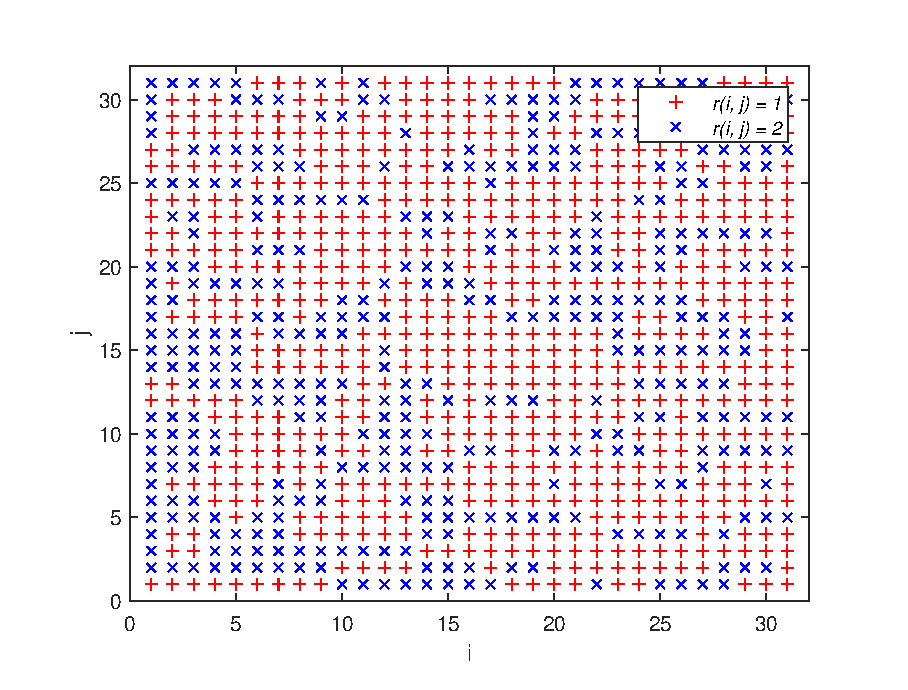
\includegraphics[scale=0.6]{./simulations/r_eps.eps}
	\caption{Modes of the considered  2D system}
	\label{fig1}
\end{figure}
\begin{figure}[!htb]
	\centering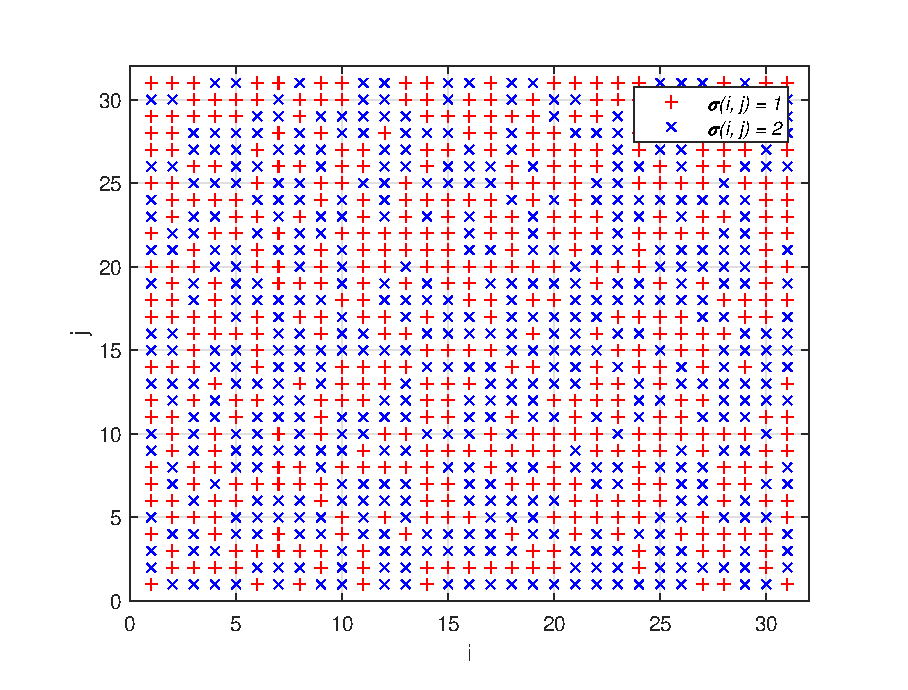
\includegraphics[scale=0.6]{./simulations/sigma_eps.eps}\\ 
	\caption{Modes of the 2D-SMC}
	\label{fig2}
\end{figure}
A possible time sequences with two different directions of the system modes and the asynchronous controller modes are depicted in Fig.\ref{fig1}-\ref{fig2}. By comparison, it is clear that the designed controller run asynchronously with the original 2D system.  \\
Based on the corresponding assumptions, the boundary condition $X_{0}$ and  exogenous disturbance $w(i,j)$ are assumed to be
\begin{equation*}
\begin{aligned}
	x^{h}(0, j)&=\begin{cases}
		0.1, \quad 0\leq j \leq 10 \\
		0, \quad \ \ elsewhere
	\end{cases} \\
	x^{v}(i, 0)&=\begin{cases}
	0.1, \quad 0\leq i \leq 10 \\
	0, \quad \ \ elsewhere
	\end{cases}\\
	w(i, j)\ &=\begin{cases}
	0.2, \quad 0\leq i,j \leq 10 \\
	0, \quad \ \ elsewhere
	\end{cases}
\end{aligned}
\end{equation*}
\begin{figure}[!htb]
\centering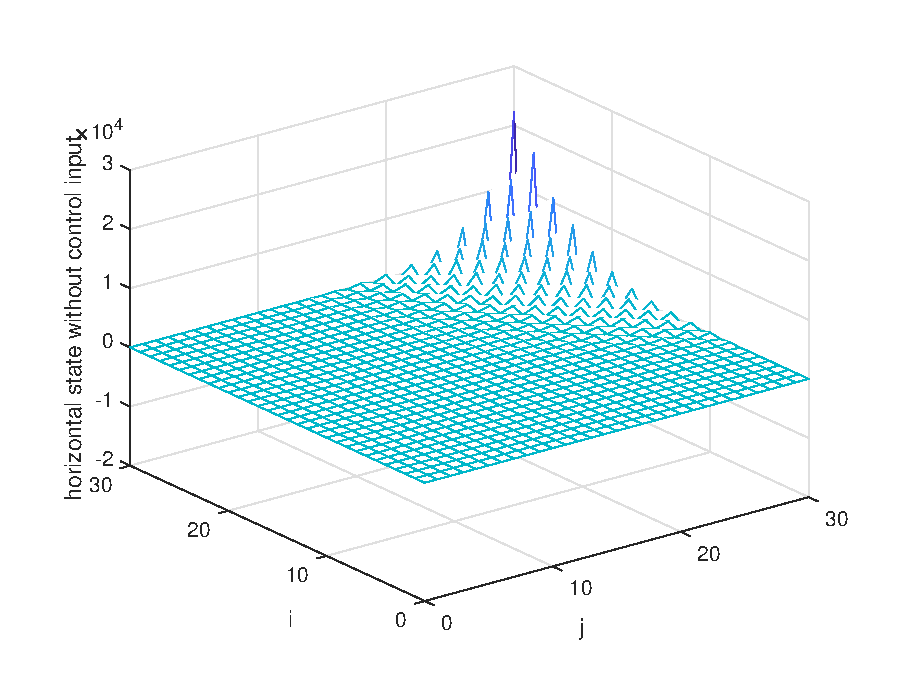
\includegraphics[scale=0.6]{./simulations/hx-no-controll-input.eps}
\caption{ Horizontal state $x^{h}(i,j)$ with $u(i,j)=0$}
\label{fig3}
\end{figure}
\begin{figure}[!htb]
\centering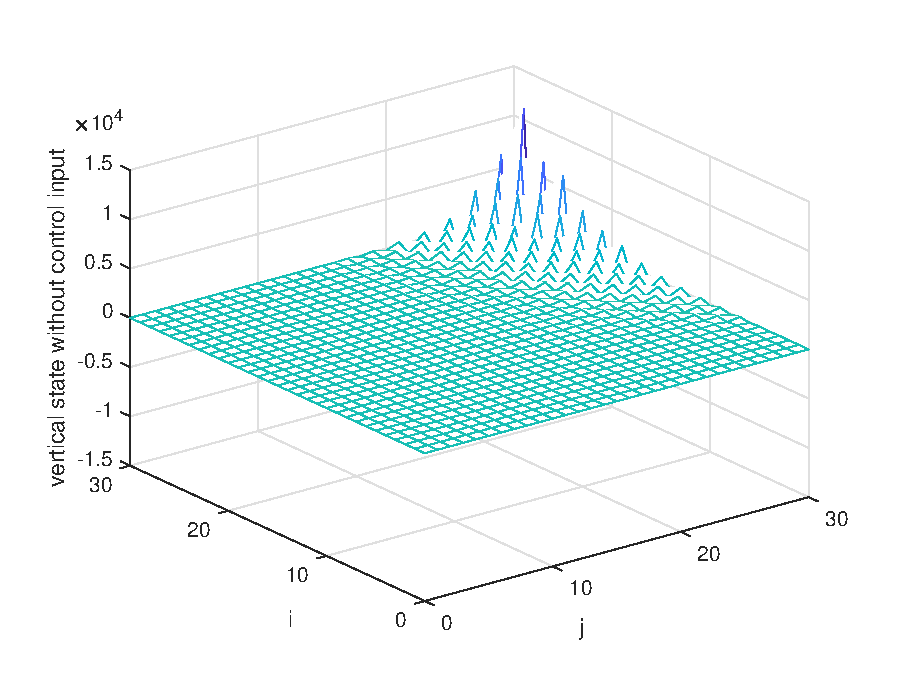
\includegraphics[scale=0.6]{./simulations/vx-no-controll-input.eps}\\ 
\caption{Vertical state $x^{v}(i,j)$ with $u(i,j)=0$}
\label{fig4}
\end{figure}
 The horizontal and vertical state responses of the open-loop system \eqref{system-equation} under $u(i,j) = 0$ are depicted in Fig.\ref{fig3} and Fig.\ref{fig4}, respectively. The obtained result implies the considered 2D system is unstable under zero control input. 
Next, let's follow the procedures of asynchronous 2D-SMC law design algorithm, and obtain the sliding model controller gain. 
Letting $\beta_{1}=0.6$ and $\beta_{2}=0.4$, then the  matrix $G$ can be calculated as follows:
\begin{equation*}
G=\begin{bmatrix}
0.2&-0.16\\
-0.02&-0.26
\end{bmatrix}
\end{equation*}
It's easy to verify that the non-singularity of the matrix $GB_{k}$ is satisfied for any $k\in\mathcal{N}_{1}$. The parameters $\varrho_{1}$ and $\varrho_{2}$ can be calculated as $\varrho_{1}=0.3$ and $\varrho_{2}=0.6872$, respectively. By solving optimization problem \eqref{optimization-problem}, we can obtain the following sliding mode controller gains\\
Mode1
\begin{equation*}
 	K_{1}=\begin{bmatrix}
 	4.4147  & -4.3512\\
 	-0.6827 &  -2.1886
 	\end{bmatrix}
\end{equation*}
Mode2
\begin{equation*}
K_{2} = 	\begin{bmatrix}
 4.3706  & -3.8453 \\
-0.6826 &  -2.3252 \\
\end{bmatrix}
\end{equation*}
with the minimum $H_{\infty}$ disturbance attenuation performance $\gamma^{*}=0.3164$. 
\begin{figure}[!htb]
	\centering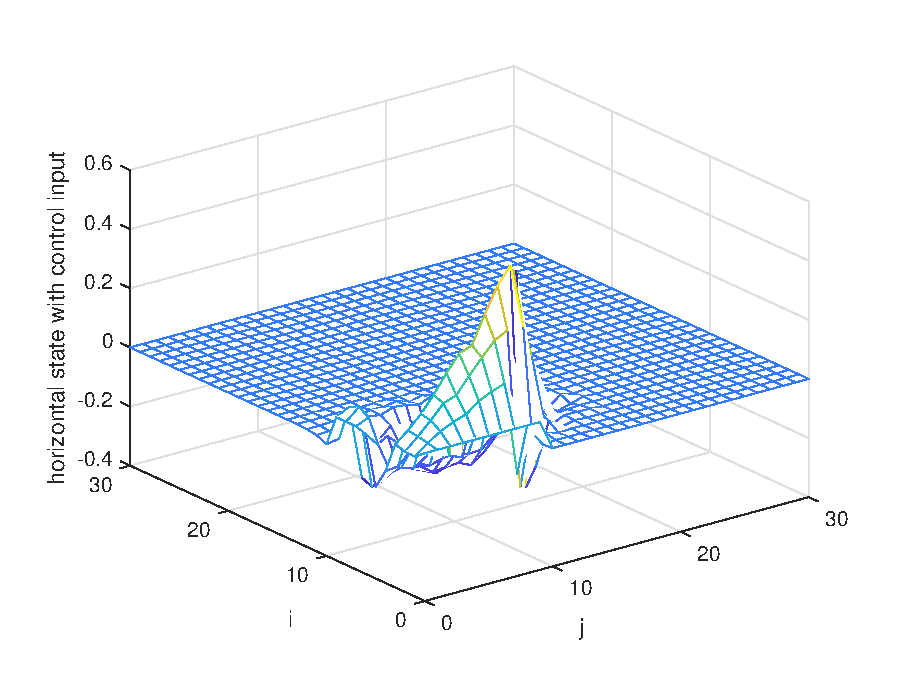
\includegraphics[scale=0.6]{./simulations/h-state-with-force.eps}
	\caption{Horizontal state $x^{h}(i,j)$ with  asynchronous 2D-SMC}
	\label{fig5}
\end{figure}
\begin{figure}[!htb]
	\centering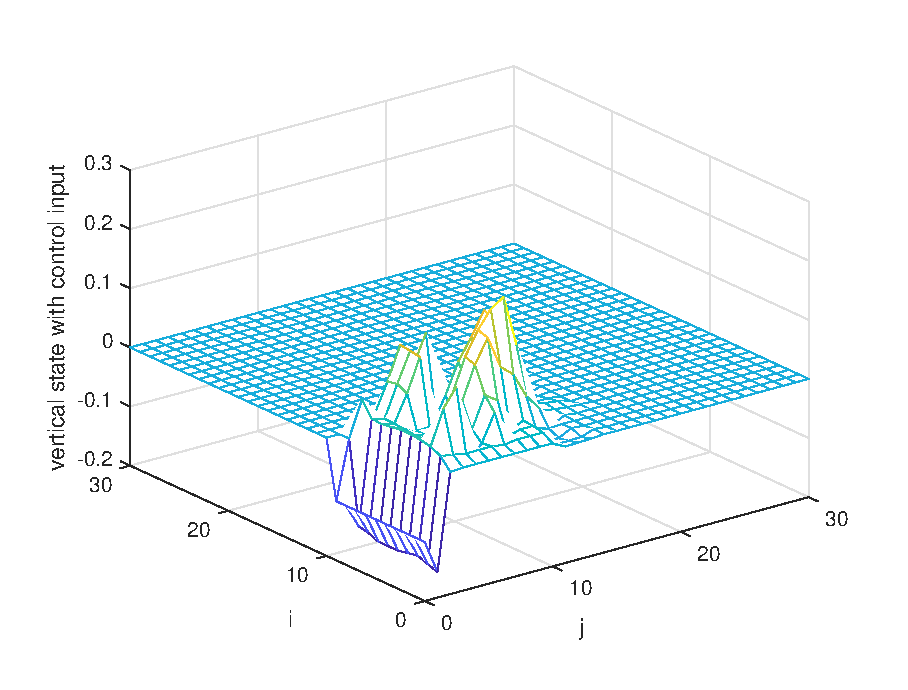
\includegraphics[scale=0.6]{./simulations/v-state-with-force_eps.eps}\\ 
	\caption{Vertical state $x^{v}(i,j)$ with asynchronous 2D-SMC}
	\label{fig6}
\end{figure}
\\The horizontal and vertical state response of the closed-loop system \eqref{closed-loop-system-equation} with asynchronous 2D-SMC law are depicted in Fig.\ref{fig5}-\ref{fig6}. It is clear that both horizontal and vertical system state converge to zero within finite steps. The sliding surface $s(i,j)$ and the asynchronous 2D-SMC law can be obtained based on the conditions given in \eqref{siding-surface-equation} and \eqref{smc-law}, respectively. Then, the horizontal 2D-SMC input, vertical 2D-SMC input, horizontal sliding surface and vertical sliding surface are depicted in Fig.\ref{fig7}-\ref{fig10}.  Clearly, the observed simulation results imply that the proposed asynchronous 2D-SMC law is effective for the considered 2D-MJS.
\begin{figure}[!htb]
	\centering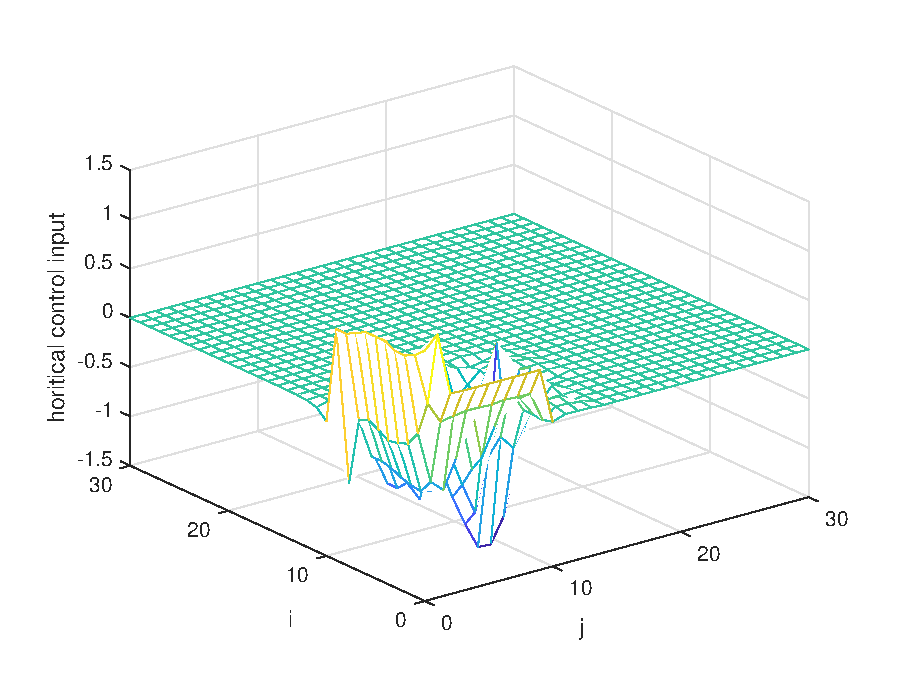
\includegraphics[scale=0.6]{./simulations/h-control-input_eps.eps}
	\caption{Horizontal  asynchronous 2D-SMC input $u^{h}(i,j)$}
	\label{fig7}
\end{figure}
\begin{figure}[!htb]
	\centering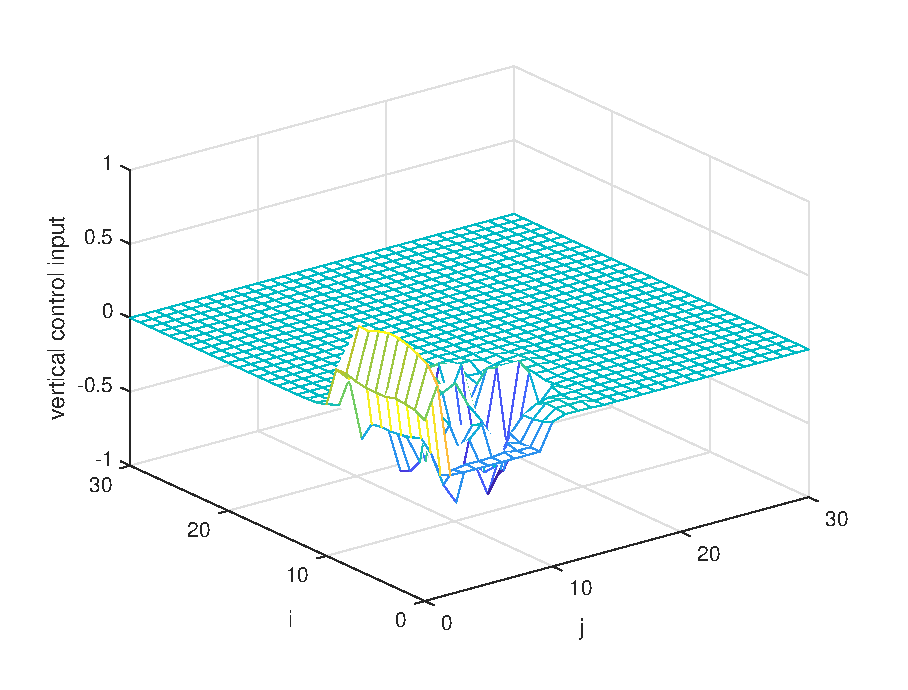
\includegraphics[scale=0.6]{./simulations/v-controll-input_eps.eps}\\ 
	\caption{Vertical asynchronous 2D-SMC input $u^{v}(i,j)$}
	\label{fig8}
\end{figure}

\begin{figure}[!htb]
	\centering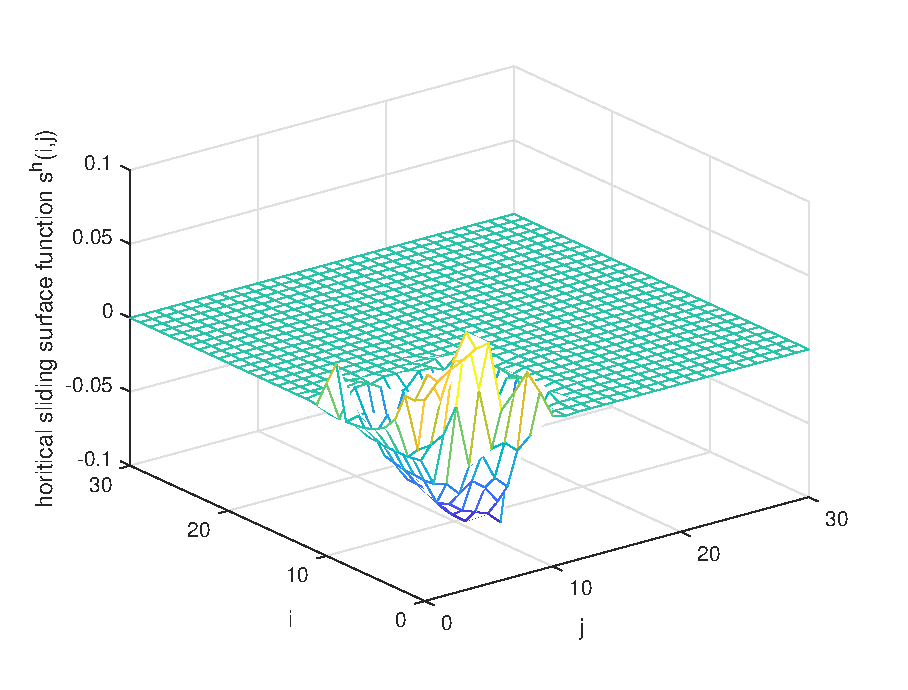
\includegraphics[scale=0.6]{./simulations/hs_eps.eps}
	\caption{Horizontal  sliding surface $s^{h}(i,j)$}
	\label{fig9}
\end{figure}
\begin{figure}[!htb]
	\centering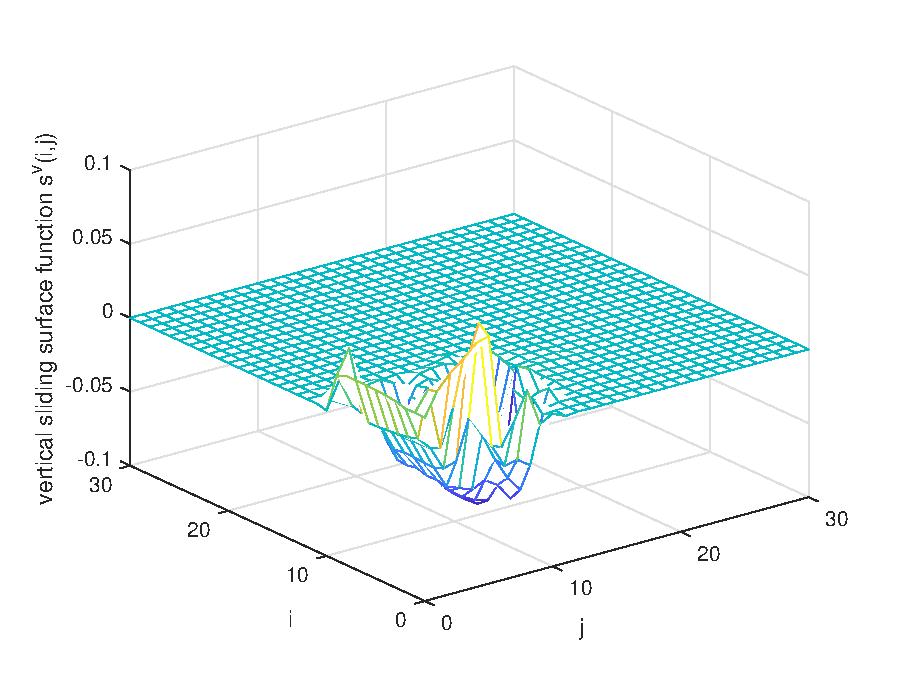
\includegraphics[scale=0.6]{./simulations/vs_eps.eps}\\ 
	\caption{Vertical sliding surface $s^{v}(i,j)$}
	\label{fig10}
\end{figure}


\section{Conclusions} \label{conclusion} 
This work has investigated the problem of asynchronous SMC for 2D-MJSs in Roesser model. In consideration that the system modes are not always accessible to the controller, an asynchronous 2D-SMC law design method is explored with hidden Markov model. By utilizing Lyapunov function, the asymptotic mean square stability for the concerned 2D-MJS  and the reachability of the sliding mode dynamics are analyzed, respectively. A sufficient condition is derived that can guarantee the concerned closed-loop 2D system is AMSS with an $H_{\infty}$ disturbance attenuation performance , and  the reachability of the 2D sliding mode dynamics is ensured simultaneously. Finally, the asynchronous SMC law design procedures are summarized as an algorithm whose effectiveness is verified by a numerical example.


\bibliographystyle{ieeetr}
\bibliography{references}

%\begin{thebibliography}{1}
%	\bibitem{costa2006discrete}
%	Costa, Oswaldo Luiz Valle, Marcelo Dutra Fragoso, and Ricardo Paulino Marques. Discrete-time Markov jump linear systems. Springer Science \& Business Media, 2006.
%	\bibitem{wu2014asynchronous}
%	Wu, Zheng-Guang, Peng Shi, Hongye Su, and Jian Chu. "Asynchronous $l_{2}-l_{\infty}$ filtering for discrete-time stochastic Markov jump systems with randomly occurred sensor nonlinearities." Automatica 50, no. 1 (2014): 180-186.
%	\bibitem{zhang2008analysis}
%	Zhang, Lixian, El-Kébir Boukas, and James Lam. "Analysis and synthesis of Markov jump linear systems with time-varying delays and partially known transition probabilities." IEEE Transactions on Automatic Control 53.10 (2008): 2458-2464.
%	\bibitem{shi2006designing}
%	Shi, Peng, Yuanqing Xia, G. P. Liu, and David Rees. "On designing of sliding-mode control for stochastic jump systems." IEEE Transactions on Automatic Control 51, no. 1 (2006): 97-103.
%	\bibitem{zhang2009stability}
%	Zhang, Lixian, and El-Kébir Boukas. "Stability and stabilization of Markovian jump linear systems with partly unknown transition probabilities." Automatica 45.2 (2009): 463-468.
%	
%	\bibitem{todorov2016new}
%	Todorov, Marcos G., and Marcelo D. Fragoso. "New methods for mode-independent robust control of Markov jump linear systems." Systems \& Control Letters 90 (2016): 38-44.
%	
%	\bibitem{wu2005mode}
%	Wu, Huai-Ning, and Kai-Yuan Cai. "Mode-independent robust stabilization for uncertain Markovian jump nonlinear systems via fuzzy control." IEEE Transactions on Systems, Man, and Cybernetics, Part B (Cybernetics) 36.3 (2005): 509-519.
%	
%	\bibitem{dolgov2017static}
%	Dolgov, M., \& Hanebeck, U. D. (2017). Static output-feedback control of Markov jump linear systems without mode observation. IEEE Transactions on Automatic Control, 62(10), 5401-5406.
%	
%	
%	\bibitem{wu2016passivity}
%	Wu, Zheng-Guang, Peng Shi, Zhan Shu, Hongye Su, and Renquan Lu. "Passivity-based asynchronous control for Markov jump systems." IEEE Transactions on Automatic Control 62, no. 4 (2016): 2020-2025.
%	
%	\bibitem{shen2019h}
%	Shen, Ying, Zheng-Guang Wu, Peng Shi, Zhan Shu, and Hamid Reza Karimi. "$H_{\infty}$ control of Markov jump time-delay systems under asynchronous controller and quantizer." Automatica 99 (2019): 352-360.
%	
%	\bibitem{zhang2017fuzzy}
%	Zhang, Meng, Peng Shi, Zhitao Liu, Hongye Su, and Longhua Ma. "Fuzzy model-based asynchronous $H_{\infty}$ filter design of discrete-time Markov jump systems." Journal of the Franklin Institute 354, no. 18 (2017): 8444-8460.
%	
%	\bibitem{dong2018hidden}
%	Dong, Shanling, Zheng-Guang Wu, Ya-Jun Pan, Hongye Su, and Yang Liu. "Hidden-Markov-model-based asynchronous filter design of nonlinear Markov jump systems in continuous-time domain." IEEE transactions on cybernetics 49, no. 6 (2018): 2294-2304.
%	
%	
%	\bibitem{du2018discrete}
%	Du, Haibo, Xiuping Chen, Guanghui Wen, Xinghuo Yu, and Jinhu Lü. "Discrete-time fast terminal sliding mode control for permanent magnet linear motor." IEEE Transactions on Industrial Electronics 65, no. 12 (2018): 9916-9927.
%	
%	\bibitem{wang2017sliding}
%	Wang, Yueying, Yabin Gao, Hamid Reza Karimi, Hao Shen, and Zhijun Fang. "Sliding mode control of fuzzy singularly perturbed systems with application to electric circuit." IEEE Transactions on Systems, Man, and Cybernetics: Systems 48, no. 10 (2017): 1667-1675.
%	
%	\bibitem{baek2016new}
%	Baek, Jaemin, Maolin Jin, and Soohee Han. "A new adaptive sliding-mode control scheme for application to robot manipulators." IEEE Transactions on Industrial Electronics 63.6 (2016): 3628-3637.
%	
%	\bibitem{edwards1998sliding}
%	Edwards, Christopher, and Sarah Spurgeon. Sliding mode control: theory and applications. Crc Press, 1998.
%	
%	\bibitem{li2015state}
%	Li, Fanbiao, Ligang Wu, Peng Shi, and Cheng-Chew Lim. "State estimation and sliding mode control for semi-Markovian jump systems with mismatched uncertainties." Automatica 51 (2015): 385-393.
%	
%	\bibitem{wu2010state}
%	Wu, Ligang, Peng Shi, and Huijun Gao. "State estimation and sliding-mode control of Markovian jump singular systems." IEEE Transactions on Automatic Control 55.5 (2010): 1213-1219.
%	
%	\bibitem{wang2017smc}
%	Wang, Yueying, Yuanqing Xia, Hao Shen, and Pingfang Zhou. "SMC design for robust stabilization of nonlinear Markovian jump singular systems." IEEE Transactions on Automatic Control 63, no. 1 (2017): 219-224.
%	
%	\bibitem{song2018asynchronous}
%	Song, Jun, Yugang Niu, and Yuanyuan Zou. "Asynchronous sliding mode control of Markovian jump systems with time-varying delays and partly accessible mode detection probabilities." Automatica 93 (2018): 33-41.
%
%	\bibitem{li2017passivity}
%	Li, Fanbiao, Chenglong Du, Chunhua Yang, and Weihua Gui. "Passivity-based asynchronous sliding mode control for delayed singular Markovian jump systems." IEEE Transactions on Automatic Control 63, no. 8 (2017): 2715-2721.
%	
%	\bibitem{qi2018observer}
%	Qi, Wenhai, Guangdeng Zong, and Hamid Reza Karim. "Observer-based adaptive SMC for nonlinear uncertain singular semi-Markov jump systems with applications to DC motor." IEEE Transactions on Circuits and Systems I: Regular Papers 65.9 (2018): 2951-2960.
%	
%	
%	\bibitem{roesser1975discrete}
%	Roesser, Robert. "A discrete state-space model for linear image processing." IEEE Transactions on Automatic Control 20.1 (1975): 1-10.
%	
%	\bibitem{marszalek1984two}
%	Marszalek, Wieslaw. "Two-dimensional state-space discrete models for hyperbolic partial differential equations." Applied Mathematical Modelling 8.1 (1984): 11-14.
%	
%	\bibitem{rogers2015multidimensional}
%	E. Rogers, K. Galkowski, W. Paszke, K. L. Moore, P. H. Bauer, L. Hladowski, and P. Dabkowski, “Multidimensional control systems: case studies in design and evaluation,” Multidimensional Systems and Signal Processing, vol. 26, no. 4, pp. 895–939, 2015.
%	
%	\bibitem{fornasini1978doubly}
%	Fornasini, Ettore, and Giovanni Marchesini. "Doubly-indexed dynamical systems: State-space models and structural properties." Mathematical systems theory 12.1 (1978): 59-72.
%	
%	\bibitem{du2001h}
%	Du, Chunling , L. Xie , and C. Zhang . "$\mathscr{H}_{\infty}$ control and robust stabilization of two-dimensional systems in Roesser models." Automatica 37.2(2001):205-211.
%	
%	\bibitem{du2002hinfinity}
%	Du, Chungling, and Lihua Xie. $H_{\infty}$ Control and Filtering of Two-Dimensional Systems. Vol. 278. Springer Science \& Business Media, 2002.
%	
%	\bibitem{trinh2016stability}
%	Trinh, Hieu. "Stability of two-dimensional Roesser systems with time-varying delays via novel 2D finite-sum inequalities." IET Control Theory \& Applications 10.14 (2016): 1665-1674.
%	
%	\bibitem{ahn2016stochastic}
%	Ahn, Choon Ki, Ligang Wu, and Peng Shi. "Stochastic stability analysis for 2-D Roesser systems with multiplicative noise." Automatica 69 (2016): 356-363.
%	
%	\bibitem{chesi2016robust}
%	Chesi, Graziano, and Richard H. Middleton. "Robust stability and performance analysis of 2D mixed continuous–discrete-time systems with uncertainty." Automatica 67 (2016): 233-243.
%	
%	\bibitem{ahn2015two}
%	Ahn, Choon Ki, Peng Shi, and Michael V. Basin. "Two-dimensional dissipative control and filtering for Roesser model." IEEE Transactions on Automatic Control 60.7 (2015): 1745-1759.
%	
%	\bibitem{liu2005adaptive}
%	Liu, Diantong, Jianqiang Yi, Dongbin Zhao, and Wei Wang. "Adaptive sliding mode fuzzy control for a two-dimensional overhead crane." Mechatronics 15, no. 5 (2005): 505-522.
%	
%	\bibitem{wu2008sliding}
%	Wu, Ligang, and Huijun Gao. "Sliding mode control of two-dimensional systems in Roesser model." IET Control Theory \& Applications 2.4 (2008): 352-364.
%	
%	\bibitem{yang2019two}
%	Yang, Rongni, and Wei Xing Zheng. "Two-dimensional Sliding Mode Control of Discrete-Time Fornasini-Marchesini Systems." IEEE Transactions on Automatic Control (2019).
%	
%	\bibitem{gao2004stabilization}
%	Gao, Huijun, James Lam, Shengyuan Xu, and Changhong Wang. "Stabilization and $H_{\infty}$ control of two-dimensional Markovian jump systems." IMA Journal of Mathematical Control and Information 21, no. 4 (2004): 377-392.
%	
%	\bibitem{wu2018hcontrol2d}
%	Wu, Zheng-Guang, Ying Shen, Peng Shi, Zhan Shu, and Hongye Su. "$H_{\infty}$ Control for 2-D Markov Jump Systems in Roesser Model." IEEE Transactions on Automatic Control 64, no. 1 (2018): 427-432.
%	
%	\bibitem{wu2008hfiltering2d}
%	Wu, Ligang, Peng Shi, Huijun Gao, and Changhong Wang. "$H_{\infty}$ filtering for 2D Markovian jump systems." Automatica 44, no. 7 (2008): 1849-1858.
%	
%	\bibitem{wu2006modelreduction}
%	Wu, Ligang, Peng Shi, Huijun Gao, and Changhong Wang. "$H_{\infty}$ mode reduction for two-dimensional discrete state-delayed systems." IEE Proceedings-Vision, Image and Signal Processing 153, no. 6 (2006): 769-784.
%	
%	
%	\bibitem{shen2019dissipativity}
%	Shen, Ying, Zheng-Guang Wu, Peng Shi, and Guanghui Wen. "Dissipativity based fault detection for 2D Markov jump systems with asynchronous modes." Automatica 106 (2019): 8-17.
%	
%	
%\end{thebibliography}




% that's all folk\tau 
\end{document}





